 \documentclass{beamer}
%
% Choose how your presentation looks.
% For more themes, color themes and font themes, see:
% http://deic.uab.es/~iblanes/beamer_gallery/index_by_theme.html
%
\mode<presentation>
{
  \usetheme{Madrid}      % or try Darmstadt, Madrid, Warsaw, ...
  \usecolortheme{seahorse} % or try albatross, beaver, crane, ...
  \usefonttheme{serif}  % or try serif, structurebold, ...
  \setbeamertemplate{navigation symbols}{}
  \setbeamertemplate{caption}[numbered]
  \usepackage{amsmath}
  \usepackage{tcolorbox}
  \usepackage[export]{adjustbox}
  \tcbuselibrary{most}
  \usepackage{arydshln}
  \usepackage{tikz}
  \usetikzlibrary{plotmarks}
  \usepackage{pgfplots}
  \usepackage{cancel}
 %\usepackage{enumitem}
%\usepackage{enumerate}
  %\usepackage[shortlabels]{enumitem}
} 


\definecolor{myblue}{RGB}{65,105,225} 
\definecolor{myorange}{RGB}{250,190,0}

\setbeamercolor{structure}{fg=white,bg=myorange}
\setbeamercolor*{palette primary}{fg=myblue,bg=myorange}
\setbeamercolor*{palette secondary}{fg=white,bg=myblue}
\setbeamercolor*{palette tertiary}{bg=myblue,fg=white}
\setbeamercolor*{palette quaternary}{fg=white,bg=myorange!50}

\setbeamercolor{frametitle}{fg=black!90!myblue}

\setbeamercolor{section in head/foot}{fg=white,bg=myblue}
\setbeamercolor{author in head/foot}{fg=black,bg=myorange}
\setbeamercolor{title in head/foot}{fg=white,bg=myblue}

\setbeamertemplate{navigation symbols}{}

\setbeamertemplate{itemize/enumerate body begin}{\large}
\setbeamertemplate{itemize/enumerate subbody begin}{\large}
\setbeamertemplate{itemize/enumerate subsubbody begin}{\large}



\defbeamertemplate*{headline}{mytheme}
{%
  \begin{beamercolorbox}[ht=2.25ex,dp=3.75ex]{section in head/foot}
    \insertnavigation{\paperwidth}
  \end{beamercolorbox}%
}%

\defbeamertemplate*{footline}{mytheme}
{
  \leavevmode%
  \hbox{%
  \begin{beamercolorbox}[wd=.5\paperwidth,ht=2.25ex,dp=1ex,right]{author in head/foot}%
    \usebeamerfont{author in head/foot}\insertshortauthor\hspace*{2em}
  \end{beamercolorbox}%
  \begin{beamercolorbox}[wd=.5\paperwidth,ht=2.25ex,dp=1ex,left]{title in head/foot}%
    \usebeamerfont{title in head/foot}\hspace*{2em}\insertshortsubtitle\hspace*{2em}
    \insertframenumber{} / \inserttotalframenumber
  \end{beamercolorbox}}%
  \vskip0pt%
}

\usepackage[english]{babel}
%\usepackage[utf8x]{inputenc}
\usepackage{xcolor}
\usepackage{listings}
\usepackage{pgf}  
\usepackage{textpos}
\usepackage{tabulary}
\usepackage{booktabs}
\usepackage{systeme, mathtools}
\usepackage{scrextend}
\usepackage{hyperref}
\usepackage{setspace}
\usepackage{rotating}
\lstset
{
    language=[LaTeX]TeX,
    breaklines=true,
    basicstyle=\tt\scriptsize,
    %commentstyle=\color{green}
    keywordstyle=\color{blue},
    %stringstyle=\color{black}
    identifierstyle=\color{magenta},
}
\newcommand{\bftt}[1]{\textbf{\texttt{#1}}}
%\newcommand{\comment}[1]{{\color[HTML]{008080}\textit{\textbf{\texttt{#1}}}}}
\newcommand{\cmd}[1]{{\color[HTML]{008000}\bftt{#1}}}
\newcommand{\bs}{\char`\\}
\newcommand{\cmdbs}[1]{\cmd{\bs#1}}
\newcommand{\lcb}{\char '173}
\newcommand{\rcb}{\char '175}
\newcommand{\cmdbegin}[1]{\cmdbs{begin\lcb}\bftt{#1}\cmd{\rcb}}
\newcommand{\cmdend}[1]{\cmdbs{end\lcb}\bftt{#1}\cmd{\rcb}}

\newcommand{\wllogo}{\textbf{Overleaf}}

% this is where the example source files are loaded from
% do not include a trailing slash
\newcommand{\fileuri}{https://raw.githubusercontent.com/GiancarloSucci/UniBo.IDSEPC.A2022/main/A2022.IDSEPCLaTeX/}


\usepackage{stackengine}
\def\Ruble{\stackengine{.67ex}{%
  \stackengine{.48ex}{\textsf{P}}{\rule{.8ex}{.12ex}\kern.6ex}{O}{r}{F}{F}{L}%
  }{\rule{.8ex}{.12ex}\kern.6ex}{O}{r}{F}{F}{L}\kern-.1ex}



%----------------------------------------------------------------------------------------
%	TITLE PAGE
%----------------------------------------------------------------------------------------
\title[L01]{Artificial Intelligence, Blockchain, e Criptovalute nello Sviluppo Software \newline\newline
Lezioni 10, 11 e 12: Fondamenti di Data Science per l'analisi dello sviluppo software} % The short title appears at the bottom of every slide, the full title is only on the title page

\author[{\tiny Giancarlo Succi }]{Giancarlo Succi\\\\ Dipartimento di Informatica -- Scienza e Ingegneria\\Universit\`{a} di Bologna\\
\bftt{g.succi@unibo.it}
} % Your name
\institute[unibo] % Your institution as it will appear on the bottom of every slide, may be shorthand to save space


\date{} % Date, can be changed to a custom date

\setbeamertemplate{navigation symbols}{}
\AtBeginSection[]
{
        \begin{frame}<beamer>{Outline}
                \tableofcontents[currentsection]
        \end{frame}
}
\begin{document}
\begin{frame}
\titlepage % Print the title page as the first slide

\end{frame}

%=============================================

\addtobeamertemplate{frametitle}{}{%
\begin{textblock*}{10mm}(-0.01mm,-0.95cm)

\includegraphics[width=0.9cm]{unibo-logo.png}
\end{textblock*}}

%=============================================
\begin{frame}
{\centerline{Content}}

\begin{itemize}
\item Linear Regression
\item Correlation and Covariance
\item Toward Inference
\end{itemize}
\end{frame}

%=============================================
%------------------------------------------------
\begin{frame}
{\centerline{Part 1}}

\begin{center}
\Huge Linear Regression
\end{center}
\end{frame}

%----------------------------------------------------------------------------------------
\begin{frame}
{\centerline{Linear Regression -- Problem 1}}

\begin{itemize}
\item Suppose that:
\begin{itemize}
\item  I want to relate two random scalar phenomena, $X$ and $Y$, to identify the relationships existing between them,
\item I can measure their values several times $i$, so I can have a set of pairs ($x_i$,$y_i$) with $i$ spanning the interval of observation, say $i \in [0 \ldots{} n-1]$
\end{itemize}
\end{itemize}

  \begin{center}
  \small
    \begin{tabular}{|c|c|c|}      
\toprule
     \textit{i} & \textbf{X} & \textbf{Y} \\
    \midrule  \textit{0} &1 & 3 \\
    \midrule  \textit{1} &2 & 4 \\
    \midrule  \textit{2} &5 & 4 \\
    \midrule  \textit{3} &6 & -1 \\
    \midrule  \textit{4} &7 & 5 \\
    \midrule  \textit{5} &9 & 8 \\
    \midrule  \textit{6} &12 & 9 \\
    \midrule  \textit{7} &13 & 9 \\
    \bottomrule
    \end{tabular}
  \end{center}
\end{frame}

\begin{frame}
{\centerline{Linear Regression -- Problem 2}}
%Define here the mathematical definition of the OLS linear regression, as the line that minimized the square error
Using a simple and common approach, I may try to build a relationship between the two phenomena.
However:
\begin{itemize}
\item  What kind of relationships I am going to look for?
\item How do I build it?
\end{itemize}

\end{frame}

\begin{frame}
{\centerline{Linear Regression -- Problem 3}}
%Define here the mathematical definition of the OLS linear regression, as the line that minimized the square error

In other words, I have this set of points:

\begin{center}
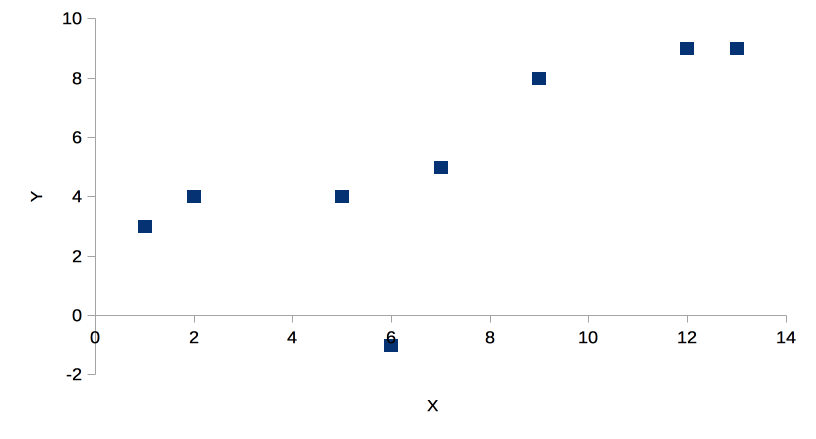
\includegraphics[width=10cm]{P2023.AIBCCSS.FoundationsDataScience/LinearRegression_Points.png}
\end{center}

\end{frame}

\begin{frame}
{\centerline{Linear Regression -- Problem 4}}
%Define here the mathematical definition of the OLS linear regression, as the line that minimized the square error

How can I build a line that represent the relationships between these two sets?

\begin{center}
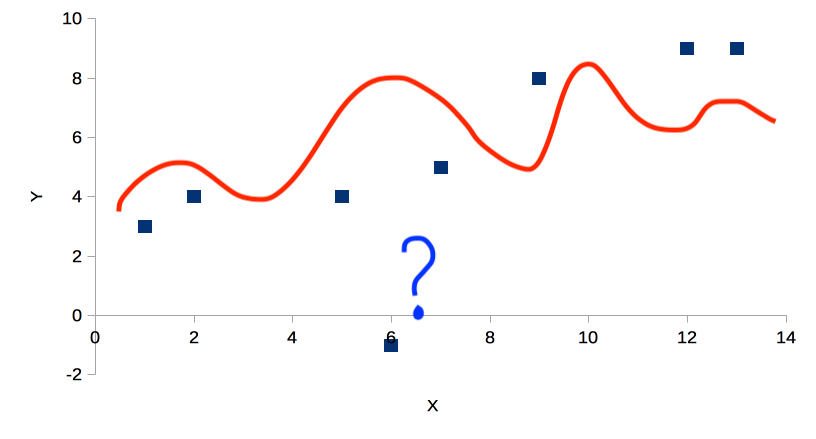
\includegraphics[width=10cm]{P2023.AIBCCSS.FoundationsDataScience/LinearRegression_Lines.png}
\end{center}



\end{frame}

%----------------------------------------------------------------------------------------
\begin{frame}
{\centerline{Linear Regression -- Definition}}
%Define here the mathematical definition of the OLS linear regression, as the line that minimized the square error
We need to define:
\begin{itemize}
\item A \textcolor{red}{mean function} that represents the relationship that I hypothesize between the phenomena $X$ and $Y$\\
\item A \textcolor{red}{cost-minimization function} to define the parameters of the mean function
\end{itemize}
We will use initially:
\begin{itemize}
\item As \textcolor{red}{mean function} the simple line\\
\item As \textcolor{red}{cost function} the square of the errors between the modeled values and the real values
\end{itemize}
We define \textcolor{red}{Ordinary Least Squares (OLS) Linear Regression} as a simple line that minimizes a square error between modelled values and real values.
\end{frame}

\begin{frame}
{\centerline{Linear Regression -- Goal}}
%Define here the mathematical definition of the OLS linear regression, as the line that minimized the square error

This is what we would like to build:

\begin{center}
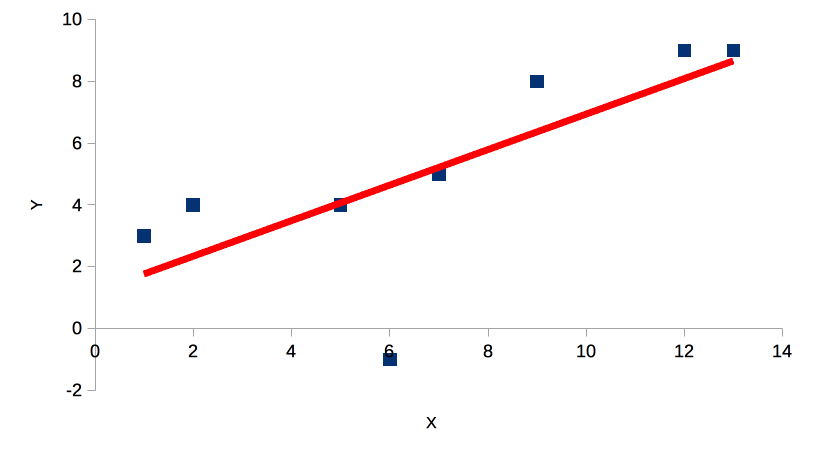
\includegraphics[width=12cm]{P2023.AIBCCSS.FoundationsDataScience/LinearRegression_OLS.png}
\end{center}



\end{frame}

\begin{frame}
{\centerline{Linear Regression -- Alternative Goal 1}}
%Define here the mathematical definition of the OLS linear regression, as the line that minimized the square error

But we could have used as a mean function a cubic function:

\begin{center}
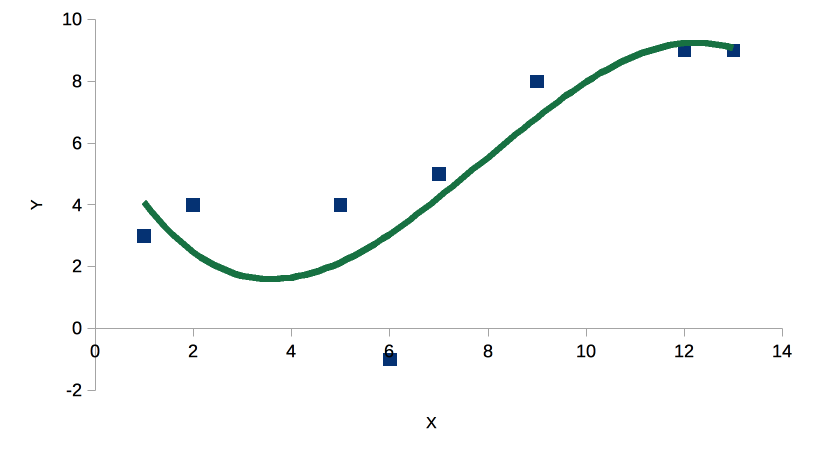
\includegraphics[width=12cm]{P2023.AIBCCSS.FoundationsDataScience/LinearRegression_Degree3.png}
\end{center}

\end{frame}

\begin{frame}
{\centerline{Linear Regression -- Alternative Goal 2}}
%Define here the mathematical definition of the OLS linear regression, as the line that minimized the square error

But we could have used as a mean function a fifth order function:

\begin{center}
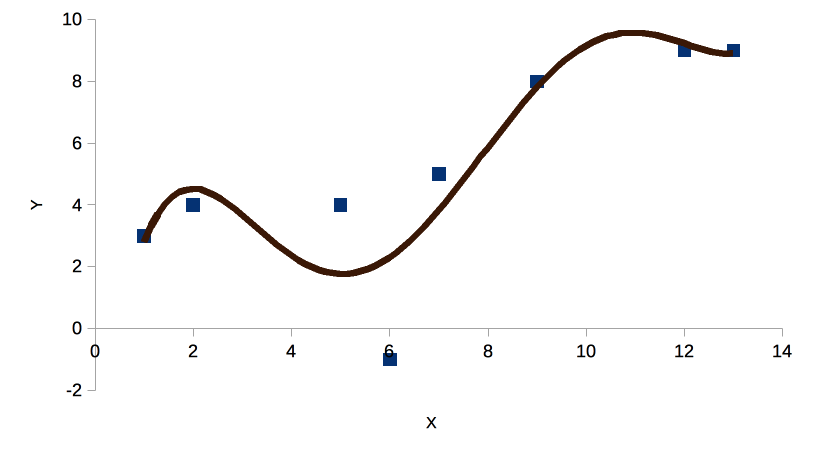
\includegraphics[width=12cm]{P2023.AIBCCSS.FoundationsDataScience/LinearRegression_Degree5.png}
\end{center}

\end{frame}

\begin{frame}
{\centerline{Linear Regression -- All Goals}}
%Define here the mathematical definition of the OLS linear regression, as the line that minimized the square error

What are the differences between all these 3?

\begin{center}
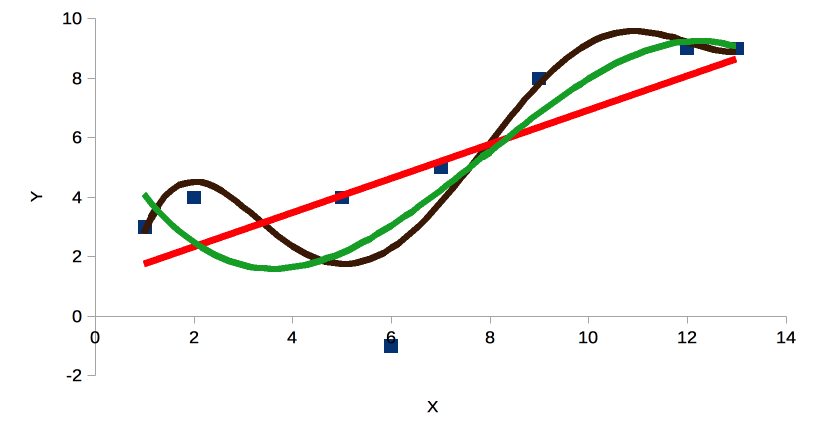
\includegraphics[width=12cm]{P2023.AIBCCSS.FoundationsDataScience/LinearRegression_O35.png}
\end{center}

\end{frame}




\begin{frame}
{\centerline{Linear Regression -- Formula (1/3)}}
I want to build a model of the kind:

$$ Y = \theta_0 + \theta_1 X $$

Where $X$ and $Y$ are the phenomena that we are measuring.\\
\vspace*{0.3cm}

Note:
\begin{itemize}
\item we know that there is no line passing for $n$ arbitrary points with $3 \leq n$
\item we need to introduce an approximation
$$ \hat{Y} = \theta_0 + \theta_1 \hat{X} + \epsilon $$
\item in our case $\epsilon$ is the error introduced by the approximation
\item as we said, our cost function, our distance from the model, will be the square of the error $\epsilon^2$
\item $ \theta_0$ and $\theta_1$ are called the \textcolor{red}{regression coefficients}
\end{itemize}

\end{frame}

\begin{frame}
{\centerline{Linear Regression -- Formula (2/3)}}
Altogether:
\begin{itemize}
\item we have a set of pairs ($x_i$,$y_i$)  with $i \in [0 \ldots{} n-1]$
\item we want to build $n$ linear equations of the kind (the mean function):
$$ y_i = \theta_0 + \theta_1 x_i + \epsilon_i $$
\item and we start with an approximation of the kind:
$$ \hat{y}_i = \theta_0 + \theta_1 x_i  $$
\end{itemize}

\end{frame}

\begin{frame}
{\centerline{Linear Regression -- Formula (3/3)}}
Altogether:
\begin{itemize}
\item our goal is to compute  $\theta_0$ and $\theta_1$ that minimize the quadratic error (the cost function)
$$ \sum_{i=0}^{n-1}\epsilon_i^2  $$

\item notice that:
\begin{itemize}
\item we will denote as ($x_i$,$y_i$) the original data
\item we will denote as ($\hat{x}_i$,$\hat{y}_i$) the approximation that we obtain in the linear regression
\item $x_i$ and $\hat{x}_i$ are the same
\item \textcolor{red}{there could be errors in the slides and you get extra credits by finding them}
\end{itemize}
\end{itemize}

\end{frame}


\begin{frame}
{\centerline{Linear Regression -- Computation}}
\begin{itemize}
\item Since 
$$ y_i = \theta_0 + \theta_1 x_i + \epsilon_i $$
\item therefore
$$\epsilon_i  = y_i - \theta_0 - \theta_1 x_i $$
\item we need to minimize:
$$ \sum_{i=0}^{n-1}\epsilon_i^2  = \sum_{i=0}^{n-1}(y_i - \theta_0 - \theta_1 x_i)^2  $$
\item we need to zero the two partial derivatives:
$$ \frac{\partial \sum_{i=0}^{n-1}(y_i - \theta_0 - \theta_1 x_i)^2}{\partial \theta_i}$$
\item so we have to solve two simple equations and then to check the Hessian
\end{itemize}

\end{frame}


\begin{frame}
{\centerline{Linear Regression -- Computation for $\theta_0$}}

$$ \frac{\partial \sum_{i=0}^{n-1}(y_i - \theta_0 - \theta_1 x_i)^2}{\partial \theta_0} =  0 \Rightarrow$$ \\
$$ 2 \sum_{i=0}^{n-1}(y_i - \theta_0 - \theta_1 x_i) = 0 \Rightarrow$$ \\
$$ \sum_{i=0}^{n-1}(y_i - \theta_0 - \theta_1 x_i) = 0 $$

\end{frame}

\begin{frame}
{\centerline{Linear Regression -- Computation for $\theta_1$}}

$$ \frac{\partial \sum_{i=0}^{n-1}(y_i - \theta_0 - \theta_1 x_i)^2}{\partial \theta_1} =  0 \Rightarrow$$ \\
$$ 2 \sum_{i=0}^{n-1}x_i(y_i - \theta_0 - \theta_1 x_i) = 0 \Rightarrow$$ \\
$$ \sum_{i=0}^{n-1}x_i(y_i - \theta_0 - \theta_1 x_i) = 0 $$

\end{frame}

\begin{frame}
{\centerline{Linear Regression -- From the first equation}}

From the first equation:

$$ \textcolor{red}{\sum_{i=0}^{n-1}(\theta_0) }= \sum_{i=0}^{n-1}( \textcolor{orange}{y_i} - \textcolor{purple}{\theta_1 x_i})  \Rightarrow $$ \\
$$ \textcolor{red}{\sum_{i=0}^{n-1}(\theta_0)} = \textcolor{orange}{\sum_{i=0}^{n-1}( y_i )} - \textcolor{purple}{\theta_1 \sum_{i=0}^{n-1}(x_i)}  \Rightarrow $$\\
$$ \textcolor{cyan}{n} \textcolor{red}{\theta_0} =  \textcolor{cyan}{n} \textcolor{orange}{\bar{y}} -  \textcolor{cyan}{n} \textcolor{purple}{\theta_1 \bar{x}}  \Rightarrow $$\\
$$ \textcolor{red}{\theta_0} = \textcolor{orange}{\bar{y}} - \textcolor{purple}{\theta_1 \bar{x} } $$



\end{frame}

\begin{frame}
{\centerline{Linear Regression -- In the second equation}}
$$ \sum_{i=0}^{n-1}x_i(\textcolor{red}{y_i} - \textcolor{orange}{\theta_0} - \textcolor{purple}{\theta_1 x_i}) = 0   \Rightarrow $$

$$ \textcolor{red}{\sum_{i=0}^{n-1}x_iy_i} - \textcolor{orange}{\theta_0 \sum_{i=0}^{n-1}x_i} - \textcolor{purple}{\theta_1 \sum_{i=0}^{n-1}x_i^2} = 0 \Rightarrow $$

$$ \textcolor{red}{\sum_{i=0}^{n-1}x_iy_i} - \textcolor{orange}{n \theta_0 \bar{x}}  - \textcolor{purple}{n \theta_1 \bar{x^2}} = 0 \Rightarrow $$


\end{frame}

\begin{frame}
{\centerline{Linear Regression -- Combining the result}}

Substituting $ \theta_0  = \bar{y} - \theta_1 \bar{x} $:

$$ \textcolor{red}{\sum_{i=0}^{n-1}x_iy_i} - \textcolor{orange}{n (\textcolor{cyan}{\bar{y} - \theta_1 \bar{x}}) \bar{x}}  - \textcolor{purple}{n \theta_1 \bar{x^2}} = 0 \Rightarrow $$

$$ \textcolor{red}{\sum_{i=0}^{n-1}x_i y_i} - \textcolor{orange}{n \textcolor{cyan}{\bar{y}}\bar{x}} + \textcolor{orange}{n \textcolor{cyan}{\theta_1 \bar{x}}^2}  - \textcolor{purple}{n \theta_1 \bar{x^2}} = 0$$


$$ \textcolor{red}{\sum_{i=0}^{n-1}x_i y_i} - \textcolor{orange}{n \bar{y}\bar{x}} + \textcolor{purple}{n \theta_1} \textcolor{cyan}{\bar{x^2}}  - \textcolor{purple}{n \theta_1} \textcolor{cyan}{\bar{x}^2}  = 0$$

$$ \textcolor{purple}{n \theta_1} (\textcolor{cyan}{\bar{x^2}}  - \textcolor{cyan}{\bar{x}^2} ) = \textcolor{red}{ \sum_{i=0}^{n-1}x_i y_i} - \textcolor{orange}{n \bar{y}\bar{x}} $$
\end{frame}

\begin{frame}
{\centerline{Linear Regression -- Final step}}

$$ \textcolor{purple}{\theta_1}  = \frac {\textcolor{red}{\sum_{i=0}^{n-1}x_i y_i} - \textcolor{orange}{n \bar{y}\bar{x}}} {\textcolor{purple}{n} (\textcolor{cyan}{\bar{x^2}}  - \textcolor{cyan}{\bar{x}^2} ) }  = \frac { \frac {\textcolor{red}{\sum_{i=0}^{n-1}x_i y_i}}{\textcolor{orange}{n}}  - \cancel{\textcolor{orange}{n}} \textcolor{orange}{\bar{y}\bar{x}}} {  \cancel{\textcolor{purple}{n}} (\textcolor{cyan}{\bar{x^2}}  - \textcolor{cyan}{\bar{x}^2} ) } = \frac { \frac {\textcolor{red}{\sum_{i=0}^{n-1}x_i y_i}}{\textcolor{orange}{n}}  - \textcolor{orange}{\bar{y}\bar{x}}} { (\textcolor{cyan}{\bar{x^2}}  - \textcolor{cyan}{\bar{x}^2} ) } $$
\vspace*{0.2cm}


$$ \theta_1  = \frac { Cov(x,y)} { Var(x) } $$

Which we can also write as:

$$\theta_1 = \frac{\sum_{i=0}^{n-1}(x_i-\bar{x})(y_i-\bar{y})}{\sum_{i=0}^{n-1}(x_i-\bar{x})^2}$$


\end{frame}

\begin{frame}
{\centerline{Going back to our exercise... }}

Using the formula above we obtain that for the following dataset:

\begin{table}[h!]
\small
  \begin{center}
    \begin{tabular}{|c|c|c|}      
    \toprule
         \textit{i} & \textbf{X} & \textbf{Y} \\
    \midrule    \midrule
	\textit{0} &1 & 3 \\
	\textit{1} &2 & 4 \\
	\textit{2} &5 & 4 \\
	\textit{3} &6 & -1 \\
	\textit{4} &7 & 5 \\
	\textit{5} &9 & 8 \\
	\textit{6} &12 & 9 \\
	\textit{7} &13 & 9 \\ \bottomrule
    \end{tabular}
  \end{center}
\end{table}


We have an equation:
$$ \hat{Y} = \theta_0 + \theta_1 \hat{X} $$
with:
\begin{itemize}
\item $\theta_0$ = 1.179 and  $\theta_1$ = 0.574

\end{itemize}

\end{frame}

\begin{frame}
{\centerline{Our model }}


\begin{table}[h!]
\small
  \begin{center}
    \begin{tabular}{|c|c|c|c|c|}      
    \toprule
     \textit{i} & \textbf{X} & \textbf{Y} & \textbf{$\hat{Y}$} & \textbf{$\epsilon$}\\
    \midrule    \midrule
	\textit{0} &1 & 3 & 1.753 & 1.247 \\
	\textit{1} &2 & 4 & 2.327 & 1.673 \\
	\textit{2} &5 & 4  & 4.049 & -0.049\\
	\textit{3} &6 & -1 & 4.623 & -5.623 \\
	\textit{4} &7 & 5  & 5.197 & -0.197\\
	\textit{5} &9 & 8  & 6.345 & 1.655\\
	\textit{6} &12 & 9  & 8.067 & 0.933\\
	\textit{7} &13 & 9  & 8.641 & 0.359\\ \bottomrule
    \end{tabular}
  \end{center}
\end{table}


\end{frame}

\begin{frame}
{\centerline{Linear Regression -- Exercise}}

Build a linear regression for the following dataset:
\begin{center}
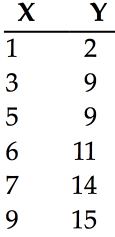
\includegraphics[width=2cm]{P2023.AIBCCSS.FoundationsDataScience/points-1.png}
\end{center}

\end{frame}
%=====%=====%=====%=====%=====%=====%=====%=====%=====
\begin{frame}
{\centerline{Linear Regression -- Exercise}}

\begin{center}
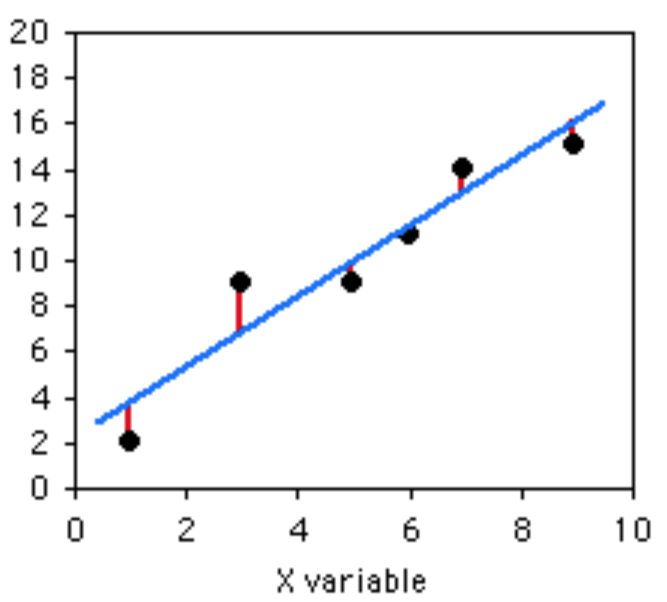
\includegraphics[width=6cm]{P2023.AIBCCSS.FoundationsDataScience/points-2.png}   
\end{center}


\end{frame}




\begin{frame}
{\centerline{Linear Regression -- Exercise}}

The regression equation for these numbers is $\hat{y}=2.0286+1.5429x$. Now, fill the blanks using such equation and calculate the sum of squared deviations (last column).
\small
\begin{table}[]
\centering
\begin{tabular}{l | l | l | l| l} 
\toprule
x & y & Predicted y ($\hat{y}$) & Deviate from predicted (abs.) & Squared deviate \\
\midrule
1 & 2 &  &  &  \\
3 & 9 &  &  &  \\
5 & 9 &  &  &  \\
6 & 11 &  &  &  \\
7 & 14 & &  &  \\
9 & 15 &  &  &  \\

\bottomrule

\end{tabular}
\end{table}
\end{frame}

%=====%=====%=====%=====%=====%=====%=====%=====%=====

\begin{frame}
{\centerline{Linear Regression -- Exercise}}

Results. The sum of squared deviations: 10.8
\small
\begin{table}[]
\centering
\begin{tabular}{l | l | l | l| l} 
\toprule
x & y & Predicted y ($\hat{y}$) & Deviate from predicted (abs.) & Squared deviate \\
\midrule

1 & 2 & 3.57 & 1.57 & 2.46 \\
3 & 9 & 6.66 & 2.34 & 5.48 \\
5 & 9 & 9.74 & 0.74 & 0.55 \\
6 & 11 & 11.29 & 0.29 & 0.08 \\
7 & 14 & 12.83 & 1.17 & 1.37 \\
9 & 15 & 15.91 & 0.91 & 0.83 \\

\bottomrule

\end{tabular}
\end{table}
\end{frame}


\begin{frame}
{\centerline{Linear Regression -- Modeling}}
In fact, we might think to use linear regression to model phenomena, assuming a linear dependence between input (the collected parameters) and output. 

Here are some “real world” examples (w.r.t. certain assumptions):

\begin{itemize}
\item Impact of SAT Score (or GPA) on College Admissions;
\item Impact of product price on number of sales;
\item Impact of rainfall amount on the number of fruits yielded;
\item Impact of blood alcohol content on coordination.
\end{itemize}

\end{frame}

\begin{frame}
{\centerline{Linear Regression -- Evaluation}}
We can evaluate the quality of linear regression, i.e. assess how good the model for the data that we have:

\begin{itemize}
\item by the sum of squares of residuals;
\item by the coefficient of determination.
\end{itemize}



\end{frame}


\begin{frame}
{\centerline{The sum of squared errors}}

The sum of squares of residuals, also called the residual sum of squares:

$$SS_{res} = \sum_i (y_i - \hat{y}_i)^2$$

In the case above $SS_{res}$ is equal to 39.751672.

\end{frame}

\begin{frame}
{\centerline{The coefficient of determination ($R^2$)}}

The coefficient of determination describes the proportion of variance of the dependent variable explained by the regression model. If the regression model is ``perfect,'' $SS_{res}$ is zero, and $R^2$ is 1.

$$R^2 = 1 - \frac{SS_{res}}{SS_{tot}}$$

The total sum of squares:

$$SS_{tot} = \sum_i (y_i - \bar{y})^2$$

where 
$$\bar{y}=\frac{1}{n}\sum_{i=1}^n y_i$$

\end{frame}

\begin{frame}
{\centerline{In the example above}}

$$SS_{tot} = \sum_i (y_i - \bar{y})^2 = 82.875 $$

Remember that:

$$SS_{res} = \sum_i (y_i - \hat{y}_i)^2 = 39.751672$$

Therefore:

$$R^2 = 1 - \frac{SS_{res}}{SS_{tot}} = 1 - \frac{39.751672}{82.875} =  0.5203$$

\end{frame}

\begin{frame}
{\centerline{Coefficient of determination ($R^2$)}}


\begin{center}
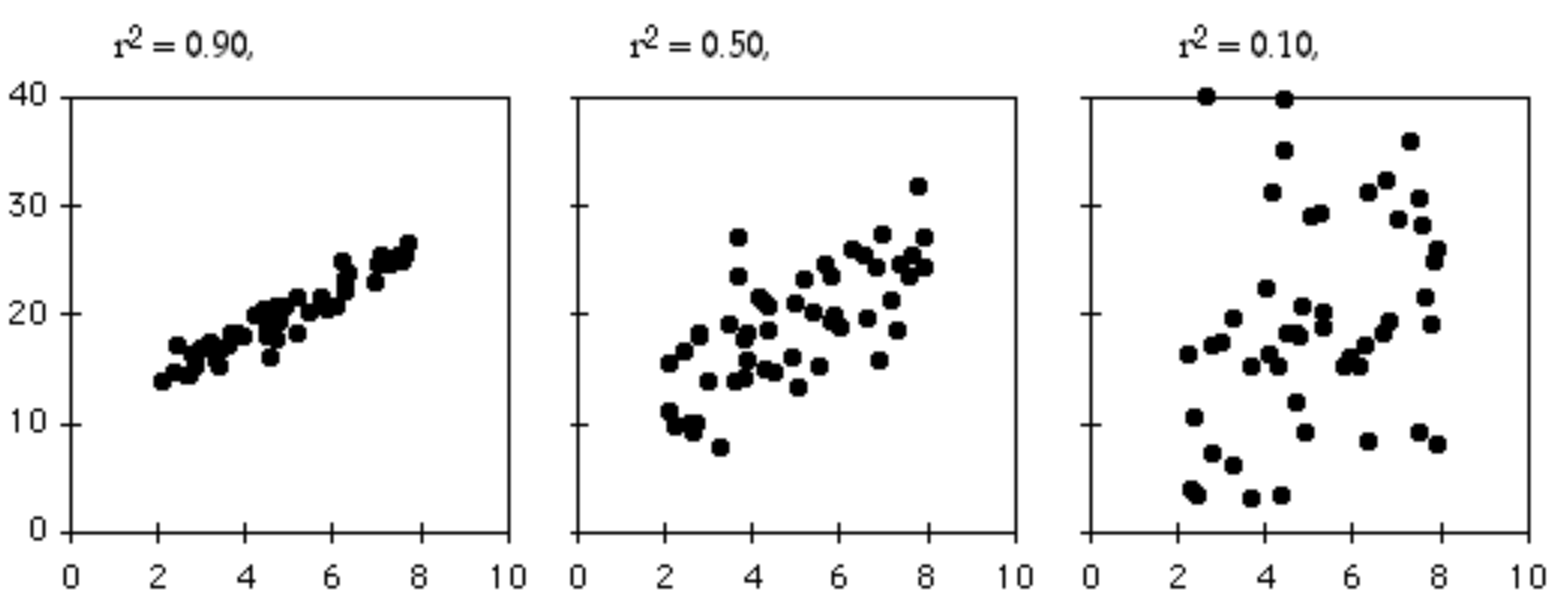
\includegraphics[width=12cm]{P2023.AIBCCSS.FoundationsDataScience/r2.png}   
\end{center}
\end{frame}

\begin{frame}
{\centerline{Multivariate Linear Regression }}

\begin{itemize}
\item The ``X'' variable is often called ``feature'' in machine learning.
\item Indeed, we could have multiple features, say, $n$.
\item If we also have $m$ observations, we could build a system of $m$ equations of the kind:
$$ y_i = \boldsymbol \theta^T \cdot \boldsymbol x_i + \epsilon_i, i=1\ldots m$$
\item and then we will build our linear regression (approximation) as:
$$ \hat{y_i} = \boldsymbol \theta^T \cdot \boldsymbol{\hat{x_i}}, i=1\ldots m$$

\item where $\boldsymbol x_i$ and  $\boldsymbol{\hat{x_i}}$-- are vectors of $n+1$ features for the i-th observation
\end{itemize}

\textcolor{red}{\textbf{Question:} Why here we use $n+1$?}
\end{frame}

\begin{frame}
{\centerline{A closed-form solution of Linear Regression }}

To find the value of $\boldsymbol \theta$, there is a closed-form solution, a mathematical equation that gives the result directly.  

This is called the \textbf{Normal Equation}:

$$\theta = (\boldsymbol X \cdot \boldsymbol X^T)^{-1} \cdot \boldsymbol X^T \cdot \boldsymbol y$$


\end{frame}

\begin{frame}
{\centerline{Derivation of the closed-form solution  (1/4) }}

\begin{itemize}
\item We start considering a set of $m$ equations of the form:
$$ \hat{y_i} = \boldsymbol \theta^T \boldsymbol x_i, i=1\ldots m$$
where $\boldsymbol x_i$ has dimension $n+1$
\item We move all the model in matrix format:
$$  \hat{\boldsymbol y} = \boldsymbol X \cdot \boldsymbol \theta   $$
\item   \textcolor{cyan}{Notice that $\hat{\boldsymbol y}$ and $\boldsymbol y$ have dimension (m,1), $\boldsymbol X$ (m,n+1), and $\theta$  (n+1,1). $\boldsymbol X \cdot \boldsymbol \theta$ has therefore dimension (m,1) as it should be.}

\item The error vector $ {\boldsymbol \epsilon}$ is defined for each pair as:

$$ {\boldsymbol \epsilon} = \hat{\boldsymbol y} - \boldsymbol y = \boldsymbol X \cdot \boldsymbol \theta - {\boldsymbol y} $$

\item And the square of the error is:
$$  (\boldsymbol X \cdot \boldsymbol \theta - \boldsymbol y)^T (\boldsymbol X \cdot \boldsymbol \theta - \boldsymbol y) $$

\end{itemize}

\end{frame}

\begin{frame}
{\centerline{Derivation of the closed-form solution  (2/4) }}

\begin{itemize}
\item To determine the values of the parameters we take the partial derivatives and we null them:
$$ \frac{ \partial  (\boldsymbol X \cdot \boldsymbol \theta - \boldsymbol y)^T (\boldsymbol X \cdot \boldsymbol \theta - \boldsymbol y)} { \partial \boldsymbol \theta} = 0 $$
\item Now we evaluate:
$$ \frac{ \partial  (\boldsymbol X \cdot \boldsymbol \theta - \boldsymbol y)^T (\boldsymbol X \cdot \boldsymbol \theta - \boldsymbol y)} { \partial \boldsymbol \theta} = $$
 $$ = \frac{\partial (
 (\boldsymbol X \cdot \boldsymbol \theta)^T (\boldsymbol X \cdot \boldsymbol \theta) -
 (\boldsymbol X \cdot \boldsymbol \theta)^T \boldsymbol y -
 \boldsymbol y^T\boldsymbol X \cdot \boldsymbol \theta +
  \boldsymbol y^T \boldsymbol y
 )}
 { \partial \boldsymbol \theta} = $$
  $$ = \frac{\partial (
 (\boldsymbol X \cdot \boldsymbol \theta)^T (\boldsymbol X \cdot \boldsymbol \theta) -
 2 (\boldsymbol X \cdot \boldsymbol \theta)^T \boldsymbol y +
  \boldsymbol y^T \boldsymbol y
 )}
 { \partial \boldsymbol \theta} $$

\end{itemize}

\end{frame}

\begin{frame}
{\centerline{Derivation of the closed-form solution  (3/4) }}

\begin{itemize}
\item Now we can consider that:
  $$ \frac{\partial (  \boldsymbol y^T \boldsymbol y )}
 { \partial \boldsymbol \theta} = 0 \text{~~~~and~~~~}   \frac{\partial (
  (\boldsymbol X \cdot \boldsymbol \theta)^T \boldsymbol y
 )}
 { \partial \boldsymbol \theta} = \boldsymbol X^T \boldsymbol y  $$
 \item \textcolor{red}{Notice that $\boldsymbol X^T \boldsymbol y$ has dimension (n+1,m) $\cdot$ (m,1), that is, (n+1,1).}

 \item We can finally conclude that:
  $$ \frac{\partial (
 (\boldsymbol X \cdot \boldsymbol \theta)^T (\boldsymbol X \cdot \boldsymbol \theta) )}
 { \partial \boldsymbol \theta} = 2  \boldsymbol X^T  \boldsymbol X \boldsymbol \theta $$
 \item \textcolor{red}{Notice that $\boldsymbol X^T \boldsymbol X \boldsymbol \theta$ has dimension (n+1,m) $\cdot$ (m,n+1)  $\cdot$ (n+1,1), that is, (n+1,1) as it should be.}

\end{itemize}

\end{frame}

\begin{frame}
{\centerline{Derivation of the closed-form solution (4/4) }}

\begin{itemize}
\item Substituting the results in the original formula:
  $$ 2  \boldsymbol X^T  \boldsymbol X \boldsymbol \theta - 2 \boldsymbol X^T \boldsymbol y = 0 \Rightarrow $$
  
    $$ \boldsymbol X^T  \boldsymbol X \boldsymbol \theta = \boldsymbol X^T \boldsymbol y  \Rightarrow $$
    
  \item Notice that $\boldsymbol X^T \boldsymbol X $ has dimension (n+1,m) $\cdot$ (m,n+1), that is, (n+1,n+1). Notice that m $\gg$ n, so we \textit{hope} that $\boldsymbol X^T \boldsymbol X $ is invertible.

    
        $$ \boldsymbol \theta = (\boldsymbol X^T  \boldsymbol X)^{-1}  \boldsymbol X^T \boldsymbol y  $$
        
\item QED.

\end{itemize}

\end{frame}

%--------------%%--------------%%--------------%%--------------%%--------------%%--------------%


% \begin{frame}
% {\centerline{\small  Linear Regression -- Computational complexity}}
% Discuss the computational complexity of linear regression
% \end{frame}


% \begin{frame}
% {\centerline{Linear Regression -- Approximation}}
% Discuss gradient descent
% \end{frame}

%--------------%%--------------%%--------------%%--------------%%--------------%%--------------%

\begin{frame}
{\centerline{Computational complexity}}

The Normal Equation computes the inverse of $X^T \cdot X$, which is an n x n matrix (where n is the number of features). 
\newline

The computational complexity of inverting such a matrix is typically about $O( n^{2.4})$ to $O( n^3)$ (depending on the implementation). 
\newline

In other words, if you double the number of features, you multiply the computation time by roughly $2^{2.4} = 5.3$ to $2^3 = 8$.

\end{frame}
%--------------%%--------------%%--------------%%--------------%%--------------%%--------------%

%--------------%%--------------%%--------------%%--------------%%--------------%%--------------%

\begin{frame}
{\centerline{Linear Regression -- Approximation}}

\textbf{Gradient Descent} is a very generic optimization algorithm capable of finding optimal solutions to a wide range of problems. The general idea of Gradient Descent is to tweak parameters iteratively in order to minimize a cost function.

\begin{center}
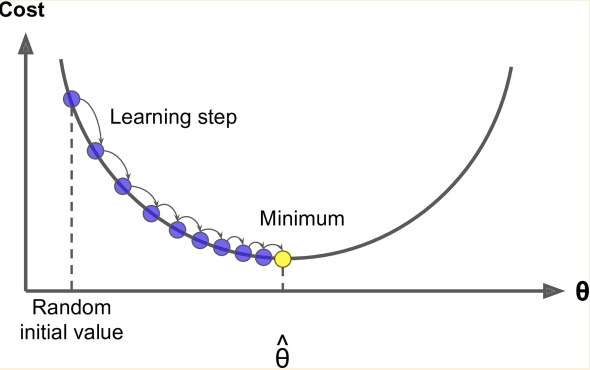
\includegraphics[width=8cm]{P2023.AIBCCSS.FoundationsDataScience/gd-1.png}
\end{center}


\end{frame}
%--------------%%--------------%%--------------%%--------------%%--------------%%--------------%

%--------------%%--------------%%--------------%%--------------%%--------------%%--------------%

\begin{frame}
{\centerline{Gradient Descent -  Computation }}

To implement Gradient Descent, you need to compute the gradient of the MSE cost function with regards to each model parameter $\theta_j$.

Mean squared error (MSE) cost function for a Linear Regression model:

$$MSE (\theta) = \frac{1}{m}\sum_{k=1}^{m} (\boldsymbol \theta^T \cdot \boldsymbol x^{(k)} - \boldsymbol y^{(k)})^2$$

$x^{(k)}$ - k-th observation vector ($x^{(k)}$ is an n-dimensional vector)



\end{frame}
%--------------%%--------------%%--------------%%--------------%%--------------%%--------------%


\begin{frame}
{\centerline{Gradient Descent -  Computation }}


To implement Gradient Descent, you need to compute the gradient of the MSE cost function with regards to each model parameter $\theta_j$.

$$\frac{\partial}{\partial \theta_j}MSE(\theta) = \frac{2}{m} \sum_{i=1}^{m}(\theta^T \cdot \boldsymbol x^{(i)} - \boldsymbol y^{(i)}  ) x_j^{(i)}$$
\end{frame}
%--------------%%--------------%%--------------%%--------------%%--------------%%--------------%

%--------------%%--------------%%--------------%%--------------%%--------------%%--------------%

\begin{frame}
{\centerline{Gradient Descent -  Computation  }}
In vector form:

$$\nabla_{\theta} MSE(\theta) = \frac{2}{m} \boldsymbol X^T (\boldsymbol X \cdot \boldsymbol \theta - \boldsymbol y)$$

We update vector $\boldsymbol \theta$ step by step:
$$\boldsymbol \theta^{next} = \boldsymbol \theta - \eta \nabla_{\theta} MSE(\theta) $$

$\eta$ -- learning rate
\end{frame}
%--------------%%--------------%%--------------%%--------------%%--------------%%--------------%



\begin{frame}
{\centerline{Learning rate}}

\begin{center}
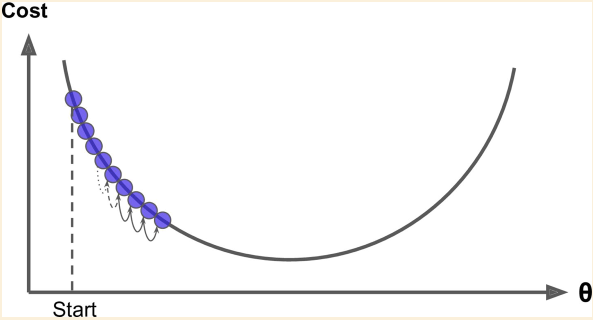
\includegraphics[width=6cm]{P2023.AIBCCSS.FoundationsDataScience/gd-2.png}
\end{center}



\begin{center}
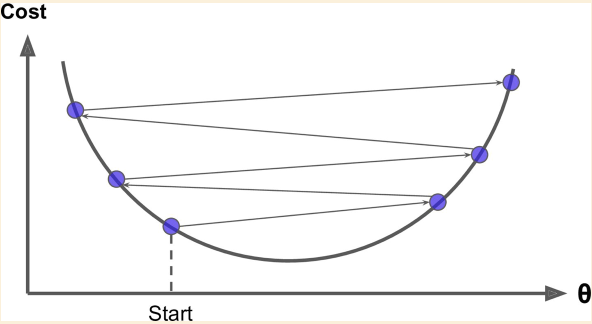
\includegraphics[width=6cm]{P2023.AIBCCSS.FoundationsDataScience/gd-3.png}
\end{center}



\end{frame}
%--------------%%--------------%%--------------%%--------------%%--------------%%--------------%
\begin{frame}
{\centerline{Pitfalls of Gradient Descent }}
\begin{center}
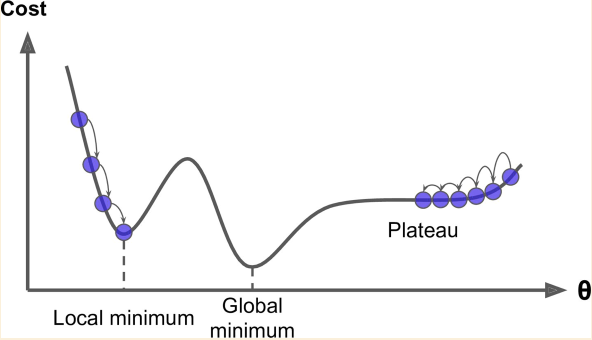
\includegraphics[width=8cm]{P2023.AIBCCSS.FoundationsDataScience/gd-4.png}
\end{center}
\end{frame}
% %--------------%%--------------%%--------------%%--------------%%--------------%%--------------%



% \begin{frame}
% {\centerline{}}

% \end{frame}

%--------------%%--------------%%--------------%%--------------%%--------------%%--------------%
\begin{frame}
{\centerline{Linear Regression and Machine Learning}}
Linear Regression is a statistical model developed in the field of Regression Analysis.

Later it was borrowed for the use of Machine Learning field.

\begin{table}[]
\centering
\caption{\textbf{Terminology difference}}
\begin{tabular}{|l|l|}
\toprule
\textbf{Regression analysis} & \textbf{Machine Learning} \\ \midrule
estimation, fitting          & training, learning         \\ \midrule
regressors                   & features                   \\ \midrule
response                     & target                    \\ \bottomrule
\end{tabular}
\end{table}

\end{frame}


\begin{frame}
{\centerline{References}}

1) \url{http://www.cs.umd.edu/~djacobs/CMSC426/Convolution.pdf}
\newline 

2) \url{https://www.researchgate.net/post/Difference\_between\_convolution\_and\_correlation}
\newline 

3) \url{https://www.tutorialspoint.com/signals\_and\_systems/convolution\_and\_correlation.htm}

\end{frame}

\begin{frame}
{\centerline{Part 2}}

\begin{center}
\Huge Correlation and Covariance
\end{center}
\end{frame}


\begin{frame}
{\centerline{Content}}

\begin{itemize}
\item Covariance
\item Correlation (aka Pearson product-moment correlation coefficient)
\item Relationship between Pearson correlation and linear regression
\end{itemize}
\end{frame}


\begin{frame}
{\centerline{Covariance}}

\begin{itemize}
\item To proceed further with our analysis we will use the concept of \textbf{covariance}, which we have already seen
\item It expresses the degree in which the variation of a random variable is connected to the variation of another random variable
\item It is defined as follows:
\begin{itemize}
\item Given two random variables $X$ and $Y$
$$Cov(X,Y) = E[ (X - E(X))(Y - E(Y))]$$
\end{itemize}
\end{itemize}

\end{frame}


\begin{frame}
{\centerline{Covariance -- graphically}}


\begin{center}
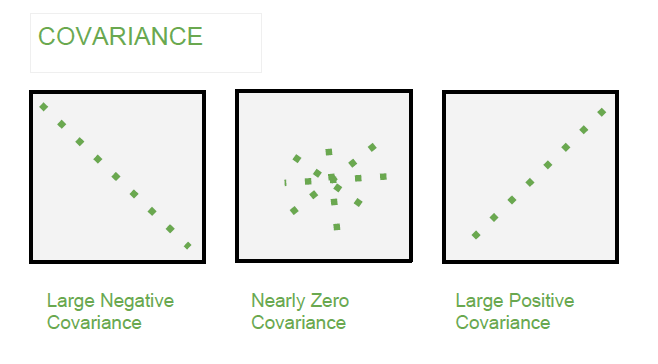
\includegraphics[width=10cm]{P2023.AIBCCSS.FoundationsDataScience/Covar.png}
\end{center} 
\begin{center}
\tiny 
Source : \url{https://www.geeksforgeeks.org/mathematics-covariance-and-correlation}
\end{center}

\end{frame}


\begin{frame}
{\centerline{About the covariance (1/2)}}

\begin{itemize}
\item We notice that:
\begin{itemize}
\item The covariance of a random variable with itself is the variance:
$$Cov(X,X) = Var(X)$$
\item There is a similar property as for the variance
$$Cov(X,Y) = E(XY) - E(X)E(Y)$$
since:
$$Cov(X,Y) = E[ (X - E(X))(Y - E(Y))] = $$
$$ = E(XY) - E(XE(Y)) - E(E(X)Y) + E(E(X)E(Y)) =$$
$$ = E(XY) - E(X)E(Y) - E(X)E(Y) + E(X)E(Y) = $$
$$ = E(XY) - E(X)E(Y)$$
QED.


\end{itemize}


\end{itemize}

\end{frame}


\begin{frame}
{\centerline{About the covariance (2/2)}} \label{P:Covariance2}

\begin{itemize}
\item The covariance is symmetric:
 $$Cov(X,Y) = Cov(Y,X)$$
\item The covariance is linear with respect to multiplications by constants:
 $$(\forall a, b \in \mathbb{R}) ~~ Cov(aX,bY) = abCov(X,Y)$$

\item If $e \sim N(0,\sigma)$, $Cov(X,e) = 0$
$$Cov(X,e) =  E(Xe) - E(X)E(e) $$
Moreover, $X$ and $e$ are independent and $E(e) = 0$\\
QED.
\end{itemize}


\end{frame}


\begin{frame}
{\centerline{Pearson Correlation Coefficient}} \label{P:Pearson}

\begin{itemize}
\item AKA Pearson product-moment correlation coefficient or just correlation coefficient
\item It expresses the linear correlation between two random variables
\item It is defined as follows:
\begin{itemize}
\item Given two random variables $X$ and $Y$
$$r_{X,Y} = \frac{Cov(X,Y)}{\sigma_X\sigma_Y}$$
\item Where:
$$\sigma_Z = \sqrt{Var(Z)}$$
\end{itemize}
\end{itemize}

\vspace*{0.5cm}

\begin{center}
\small  For the time being we intentionally ignore the difference between sample and population.
\end{center}

\end{frame}

\begin{frame}
{\centerline{Pearson Correlation Coefficient -- graphically}}


\begin{center}
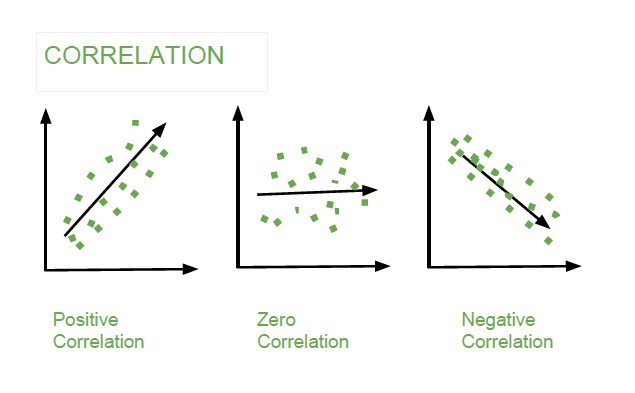
\includegraphics[width=10cm]{P2023.AIBCCSS.FoundationsDataScience/Correl.png}
\end{center} 
\begin{center}
\tiny 
Source : \url{https://www.geeksforgeeks.org/mathematics-covariance-and-correlation}
\end{center}

\end{frame}


\begin{frame}
{\centerline{About the Pearson Correlation Coefficient (1/2)}}

\begin{itemize}
\item The Pearson correlation coefficient is also often expressed as:

$$ r_{X,Y} = \frac{\sum_{i=1}^{n}(x_i-\overline{x})(y_i-\overline{y})}{\sqrt{\sum_{i=1}^{n}(x_i-\overline{x})^2\sum_{i=1}^{n}(y_i-\overline{y})^2}} $$
\item It is symmetric: $r_{X,Y} = r_{Y,X}$
\item It is invariant with respect to multiplications by, and additions of constants:\\
$(\forall a, b, c, d \in \mathbb{R} , b \neq 0, d \neq 0)~~ r_{X,Y} = r_{(a + bX),(c + dY)} $
\end{itemize}


\end{frame}

\begin{frame}
{\centerline{About the Pearson Correlation Coefficient (2/2)}}

\begin{itemize}
\item The Pearson correlation coefficient ranges from -1 to 1: $-1 \leq r_{X,Y} \leq 1$
\begin{itemize}
\item $ r_{X,Y}=1$ means perfect linear relationship
\begin{itemize}
\item all points lie on a monotonically increasing line
\end{itemize}
\item $ r_{X,Y}=-1$ means perfect opposite linear relationship
\begin{itemize}
\item all points lie on a monotonically decreasing line
\end{itemize}
\item $ r_{X,Y}= 0$ means no linear relationship between $X$ and $Y$
\end{itemize}
\end{itemize}

\end{frame}


% ============= =========== % ============= ===========
\begin{frame}
{\centerline{Back to Linear Regression (1/2)}}
\begin{itemize}
\item We now focus our attention to the case of the case of the linear regression
\item Suppose we have two phenomena that we want to measure,  $X$ and $Y$
\item Let us assume 
\begin{itemize}
\item that there is a linear relationship between them
\item that I can express the data I collect as:
$$ \boldsymbol y = \boldsymbol \theta_0 + X  \boldsymbol \theta_1 + \boldsymbol \epsilon $$
\item where $\epsilon$ is a stationary gaussian process $N(0,\sigma^2)$
\end{itemize}
\item We know the solution that minimizes the square error
\end{itemize}
\end{frame}
% ============= =========== % ============= ===========

% ============= =========== % ============= ===========
\begin{frame}
{\centerline{Back to Linear Regression (2/2)}}
\begin{itemize}
\item From this solution we have extracted the coefficient of determination
$$R^2 = 1 - \frac{SS_{res}}{SS_{tot}}$$
\item Where: 
\begin{itemize}
\item $SS_{res} = \sum_i (y_i - \hat{y}_i)^2$ 
\item \textcolor{blue}{$SS_{res} $ is the distance between the reality and the 1-degree best approximation, that is, the OLS model}
\end{itemize}
\item and
\begin{itemize}
\item $SS_{tot} = \sum_i (y_i - \overline{y})^2$
\item  \textcolor{blue}{$SS_{tot}$ is the distance between the reality and the 0-degree best approximation, that is, the mean}
\end{itemize}

\item I want to know the relationship between $R^2$ and the correlation coefficient between $X$ and $Y$, $r_{X,Y}$
\end{itemize}
\end{frame}
% ============= =========== % ============= ===========

% ============= =========== % ============= ===========
\begin{frame}
{\centerline{Our goal -- understanding R and r}}
\begin{itemize}
\item We focus on 1D
\item We are now going to prove a fundamental point.
\item Under the assumption that the noise is gaussian and centered in 0, in a linear regression:
\end{itemize}
$$R^2 = r_{X,Y}^2$$
\end{frame}
% ============= =========== % ============= ===========


% ============= =========== % ============= ===========
\begin{frame}
{\centerline{$R^2 = r_{X,Y}^2$ (1/4)}}
\begin{itemize}
\item Since
$$ \hat{y} = \theta_0 + \theta_1 x$$
\item we have from above (see page \ref{P:Pearson}) that:
$$r_{X,Y} = r_{\hat{Y},Y}$$
\item We define now the explained sum of squares (ESS) 
\begin{itemize}
\item $ ESS = \sum_i (\hat{y}_i - \overline{y})^2$
\item \textcolor{blue}{$ ESS $ is the additional knowledge we get on the random variable using a polynomial of degree 1 vs. using a polynomial of degree 0}
\end{itemize}

\item We will now prove that \textbf{under our hypotheses}:
$$ESS + SS_{res} = SS_{tot} $$
\end{itemize}
\end{frame}
% ============= =========== % ============= ===========


% ============= =========== % ============= ===========
\begin{frame}
{\centerline{ [$R^2 = r_{X,Y}^2$] -- $ESS + SS_{res} = SS_{tot} $ (1/6)}}

\begin{itemize}
\item We start from:
$$(y_{i}-{\overline {y}})=(y_{i}-{\hat {y}}_{i})+({\hat {y}}_{i}-{\overline {y}})$$

\item which we square:
$$(y_{i}-{\overline {y}})^2=(y_{i}-{\hat {y}}_{i})^2 + 2(y_{i}-{\hat {y}}_{i})({\hat {y}}_{i}-{\overline {y}}) + ({\hat {y}}_{i}-{\overline {y}})^2$$

\item and then we sum:
$$\sum_i(y_{i}-{\overline {y}})^2=\sum_i(y_{i}-{\hat {y}}_{i})^2 + \sum_i2(y_{i}-{\hat {y}}_{i})({\hat {y}}_{i}-{\overline {y}}) + \sum_i({\hat {y}}_{i}-{\overline {y}})^2$$


\end{itemize}

\begin{center}
\tiny 
Source with modifications: \url{https://en.wikipedia.org/wiki/Explained_sum_of_squares}
\end{center}

\end{frame}
% ============= =========== % ============= ===========

% ============= =========== % ============= ===========
\begin{frame}
{\centerline{ [$R^2 = r_{X,Y}^2$] -- $ESS + SS_{res} = SS_{tot} $ (2/6)}}

\begin{itemize}
\item Now we focus on:
$$\sum_i2(y_{i}-{\hat {y}}_{i})({\hat {y}}_{i}-{\overline {y}}) = 2\sum_i(y_{i}-{\hat {y}}_{i})({\hat {y}}_{i}-{\overline {y}}) $$
\item and we want to prove that it is 0, that is $\sum_i(y_{i}-{\hat {y}}_{i})({\hat {y}}_{i}-{\overline {y}}) = 0$;  considering:
$$y_i = \hat{y_i} + \epsilon_i$$
$$ E(y_i) = E(\hat{y_i} + \epsilon_i) = E(\hat{y_i}) + E(\epsilon_i) = E(\hat{y_i}) $$
because $\epsilon$ is a stationary gaussian process $N(0,\sigma^2)$

\end{itemize}

\begin{center}
\tiny 
Source with modifications: \url{https://en.wikipedia.org/wiki/Explained_sum_of_squares}
\end{center}

\end{frame}
% ============= =========== % ============= ===========

% ============= =========== % ============= ===========
\begin{frame}
{\centerline{ [$R^2 = r_{X,Y}^2$] -- $ESS + SS_{res} = SS_{tot} $ (3/6)}}

\begin{itemize}
\item We can build a system:
\[
\systeme*{
\hat{y}_i = \theta_0 + \theta_{1} x_{I},
\overline{y} = \theta_0 + \theta_1 \overline{x}
}
\]
\item from which we deduce by subtraction:
$$\textcolor{red}{\hat{y}_i - \overline{y}} = \textcolor{red}{\theta_1 (x_i - \overline{x})}$$
\item remembering that:
$$ \theta_1  = \frac { Cov(x,y)} { Var(x) } = {\frac {\sum _{i=1}^{n}(x_{i}-{\overline {x}})(y_{i}-{\overline {y}})}{\sum _{i=1}^{n}(x_{i}-{\overline {x}})^{2}}}$$
\end{itemize}

\begin{center}
\tiny
Source with modifications: \url{https://en.wikipedia.org/wiki/Explained_sum_of_squares}
\end{center}

\end{frame}

% ============= =========== % ============= ===========


% ============= =========== % ============= ===========
\begin{frame}
{\centerline{ [$R^2 = r_{X,Y}^2$] -- $ESS + SS_{res} = SS_{tot} $ (4/6)}}

\begin{itemize}
\item So:
$$\sum_i(y_{i}-{\hat {y}}_{i})({\textcolor{red}{\hat {y}_{i}-{\overline {y}}}}) = \sum_i(y_{i}-{\hat {y}}_{i})(\textcolor{red}{\theta_1 (x_i - \overline{x})})=$$
$$= \textcolor{red}{\theta_1} \sum_i\textcolor{cyan}{(y_{i}-{\hat {y}}_{i})}\textcolor{red}{(x_i - \overline{x})}$$
\item Now, let's consider that:
$$\textcolor{cyan}{(y_{i}-{\hat {y}}_{i})} = y_{i}-{\hat {y}}_{i} + \overline {y} - \overline {y} = (y_{i}-{\overline {y}})-({\hat {y}}_{i}-{\overline {y}})= $$
$$ = \textcolor{cyan}{(y_{i}-{\overline {y}})-{\theta_1}(x_{i}-{\overline {x}})}$$
\item Substituting $(y_{i}-{\hat {y}}_{i})$ above we get:
$$\textcolor{red}{\theta_1} \sum_i\textcolor{cyan}{(y_{i}-{\hat {y}}_{i})}\textcolor{red}{(x_i - \overline{x})}=\textcolor{red}{\theta_1} \sum_i\textcolor{cyan}{[(y_{i}-{\overline {y}})-{\theta_1}(x_{i}-{\overline {x}}) ]}\textcolor{red}{(x_i - \overline{x})} $$


\end{itemize}

\begin{center}
\tiny 
Source with modifications: \url{https://en.wikipedia.org/wiki/Explained_sum_of_squares}
\end{center}

\end{frame}
% ============= =========== % ============= ===========

% ============= =========== % ============= ===========
\begin{frame}
{\centerline{ [$R^2 = r_{X,Y}^2$] -- $ESS + SS_{res} = SS_{tot} $ (5/6)}}

\begin{itemize}
\item We can conclude:
$$ \theta_1 \sum_i[(y_{i}-{\overline {y}})-{\theta_1}(x_{i}-{\overline {x}}) ](x_i - \overline{x}) = $$
$$ = \theta_1 [\sum_i (y_{i}-{\overline {y}}) (x_i - \overline{x}) -
\sum_i{\theta_1}(x_{i}-{\overline {x}}) (x_i - \overline{x})] = $$
$$ = \theta_1 [\sum_i (y_{i}-{\overline {y}}) (x_i - \overline{x}) -
\sum_i{{\frac {\sum _{j}(x_{j}-{\overline {x}})(y_{j}-{\overline {y}})}{\sum _{j}(x_{j}-{\overline {x}})^{2}}}
}(x_{i}-{\overline {x}})^2] = $$


\end{itemize}

\begin{center}
\tiny 
Source with modifications: \url{https://en.wikipedia.org/wiki/Explained_sum_of_squares}
\end{center}

\end{frame}
% ============= =========== % ============= ===========

\begin{frame}
{\centerline{ [$R^2 = r_{X,Y}^2$] -- $ESS + SS_{res} = SS_{tot} $ (6/6)}}

\begin{itemize}
\item And simplifying what is in [ $\bullet$ ]:

$$ \sum_i (y_{i}-{\overline {y}}) (x_i - \overline{x}) -
\sum_i{{\frac {\sum _{j}(x_{j}-{\overline {x}})(y_{j}-{\overline {y}})}{\sum _{j}(x_{j}-{\overline {x}})^{2}}}
}(x_{i}-{\overline {x}})^2 = $$
$$=  \sum_i (y_{i}-{\overline {y}}) (x_i - \overline{x}) -
\sum _{j}(x_{j}-{\overline {x}})(y_{j}-{\overline {y}})\sum_i{{\frac {(x_{i}-{\overline {x}})^2}{\sum _{j}(x_{j}-{\overline {x}})^{2}}}
}= $$
$$=  \sum_i (x_i - \overline{x}) (y_{i}-{\overline {y}})  -
\sum _{j}(x_{j}-{\overline {x}})(y_{j}-{\overline {y}}){\frac {\sum_i{(x_{i}-{\overline {x}})^2}}{\sum _{j}(x_{j}-{\overline {x}})^{2}}} = $$
$$=  \sum_i (x_i - \overline{x}) (y_{i}-{\overline {y}})  -
\sum _{j}(x_{j}-{\overline {x}})(y_{j}-{\overline {y}}) = 0 $$


QED.


\end{itemize}

\begin{center}
\tiny 
Source with modifications: \url{https://en.wikipedia.org/wiki/Explained_sum_of_squares}
\end{center}

\end{frame}
% ============= =========== % ============= ===========


% ============= =========== % ============= ===========
\begin{frame}
{\centerline{$R^2 = r_{X,Y}^2$ (2/4)}}
\begin{itemize}
\item Now we know that, under the assumption to deal with a Gaussian noise centered in 0 we have:
$$ESS + SS_{res} = SS_{tot} $$
\item Under this hypothesis we have:
$$R^2 = 1 - \frac{SS_{res}}{SS_{tot}} = \frac{SS_{tot}-SS_{res}}{SS_{tot}} = \frac{ESS}{SS_{tot}} $$
\end{itemize}

\end{frame}
% ============= =========== % ============= ===========

% ============= =========== % ============= ===========
\begin{frame}
{\centerline{$R^2 = r_{X,Y}^2$ (3/4)}}
\begin{itemize}
\item We now consider the square of $r_{X,Y} = r_{\hat{Y},Y}$
$$r_{\hat{Y},Y}^2= \left ( \frac{Cov(\hat{Y},Y)}{\sqrt{Var(Y)Var(\hat{Y})}} \right )^2 =  \frac{Cov(\hat{Y},Y)Cov(\hat{Y},Y)}{Var(Y)Var(\hat{Y})} = $$
$$ = \frac{Cov(\hat{Y},\hat{Y} + \epsilon)Cov(\hat{Y},\hat{Y} + \epsilon)}{Var(Y)Var(\hat{Y})} = $$
$$ 
= \frac{(Cov(\hat{Y},\hat{Y})+ Cov(\hat{Y},\epsilon))(Cov(\hat{Y},\hat{Y})+ Cov(\hat{Y},\epsilon))}{Var(Y)Var(\hat{Y})} = $$
$$ 
= \frac{Cov(\hat{Y},\hat{Y})Cov(\hat{Y},\hat{Y})}{Var(Y)Var(\hat{Y})} $$


\end{itemize}

\begin{center}
\tiny 
Source with modifications: \url{https://economictheoryblog.com/2014/11/05/proof/}
\end{center}
\end{frame}

% ============= =========== % ============= ===========
% ============= =========== % ============= ===========
\begin{frame}
{\centerline{$R^2 = r_{X,Y}^2$ (4/4)}}
\begin{itemize}
\item But we know that $Cov(\hat{Y},\hat{Y}) = Var(\hat{Y})$, therefore we get that
$$r_{X,Y}^2 = \frac{Var(\hat{Y})Var(\hat{Y})}{Var(Y)Var(\hat{Y})} = \frac{Var(\hat{Y})}{Var(Y)}=$$
$$ = \frac{\frac{\sum_i{(\hat{y_i}-\overline{\hat{y}})^2}}{n}}{\frac{\sum_i(y_i-\overline{y})^2}{n}}
= \frac{{\sum_i{(\hat{y_i}-\overline{\hat{y}})^2}}}{\sum_i(y_i-\overline{y})^2} =  \frac{ESS}{SS_{tot}} $$
since we have already proven that $\overline{y} = \overline{\hat{y}}$
\end{itemize}
QED

\begin{center}
\tiny 
Source with modifications: \url{https://economictheoryblog.com/2014/11/05/proof/}
\end{center}
\end{frame}

% ============= =========== % ============= ===========

% ============= =========== % ============= ===========
\begin{frame}
{\centerline{Comment on $R^2 = r_{X,Y}^2$ }}
\begin{itemize}
\item This is a major result\\
\item It is the center of our subsequent investigation, in the case of normality of error we can model, interconnect, and understand relationships in an easy way\\
\item The next question is on how the slope of the regression line ($\theta_1$) relates to the correlation coefficient $r_{X,Y}$

\end{itemize}

\end{frame}
% ============= =========== % ============= ===========

\begin{frame}
{\centerline{$ r_{X,Y} $ and $\theta_1$}}
\begin{itemize}
\item We know that:
$$ \theta_1  = \frac { Cov(X,Y)} { Var(X) } $$
\item And that:
$$r_{X,Y} = \frac{Cov(X,Y)}{\sigma_X\sigma_Y}$$
\item Therefore:
$$ \theta_1  Var(X) = r_{X,Y}  \sigma_X\sigma_Y $$
\item We can then conclude that:
$$ \theta_1  = \frac{\sigma_X\sigma_Y}{Var(X)} r_{X,Y}   $$
$$ r_{X,Y}   = \frac{Var(X)}{\sigma_X\sigma_Y} \theta_1  $$

\end{itemize}

\end{frame}
% ============= =========== % ============= ===========

% ============= =========== % ============= ===========

\begin{frame}
{\centerline{Comment on $ r_{X,Y} ~ \sim ~ \theta_1$}}
\begin{itemize}
\item $ r_{X,Y} $ and $\theta_1$ are therefore directly and monotonically proportional
\item It means that a positive relationships implies a positive slope and viceversa
\end{itemize}

\end{frame}
% ============= =========== % ============= ===========


% https://en.wikipedia.org/wiki/Explained_sum_of_squares


\begin{frame}
{\centerline{General remark}}

\begin{itemize}
\item Right now we work with samples of larger populations of data
\item We measure properties of samples, like mean, standard deviation, covariance, correlation coefficient
\item All these properties are also random variable and have a distribution
\item Our question is therefore, what kind of distribution is the one of the correlation coefficient
\item Knowing its distribution allows us to understand the relationships existing between the variables it connect
\end{itemize}


\end{frame}

\begin{frame}
{\centerline{Part 3}}

\begin{center}
\Huge Toward Inference
\end{center}
\end{frame}

\begin{frame}
{\centerline{Content}}

\begin{itemize}
\item Premises of the Law of Large Numbers
\item Markov's inequality
\item Chebyshev’s inequality
\item Proof of the Law of Large Numbers
\item Central Limit Theorem in the Linderberg-L\'{e}vy formulation
\item Moment
\item Moment generating function
\item Proof of the Central Limit Theorem in the Linderberg-L\'{e}vy formulation
\end{itemize}


\end{frame}


\begin{frame}
{\centerline{Last words...}}

\begin{itemize}
\item Right now we work with samples of larger populations of data
\item We measure properties of samples, like mean, standard deviation, covariance, correlation coefficient
\item All these properties are also random variable and have a distribution
\item Our question is therefore, what kind of distribution is the one of the correlation coefficient
\item Knowing its distribution allows us to understand the relationships existing between the variables it connect
\end{itemize}


\end{frame}

\begin{frame}
{\centerline{Knowing the sample $\ldots$}}

\begin{itemize}
\item What can we infer of populations now that I know the properties of the sample?
\item Now we know the mean, the standard deviation, the distribution of the sample, what would be the mean, the standard deviation, and the distribution of the population?
\item Moreover, from two samples we can build a regression, what would be the regression of the population? 
\end{itemize}

\end{frame}

\begin{frame}
{\centerline{We start from the mean}}

\begin{itemize}
\item We suppose that we have an unknown population $\mathfrak{P}$ of entities on a ratio scale from which we extract $n$ samples $\mathfrak{S}_i$ with $i \in [1 \ldots{} n]$
\item Each sample $i$ is composed by $\mathfrak{n_i}$ elements $e_{i,j}$ with $j \in [1\ldots{}\mathfrak{n_i}]$
\item We can compute the set of the means of each sample $\mathfrak{S}_i$, $\mathfrak{m}_i$ with $i \in [1 \ldots{} n]$
\item $\mathfrak{m}_i$ is a random variable, so we would like to know what is its structure
\item There are two fundamental theorems about the distributions of such  $\mathfrak{m}_i$, the Law of Large Numbers (LLN) and the Central Limit Theorem (CLT)
\item Since we are not making \textbf{any} assumption on the population  $\mathfrak{P}$, we ignore it and consider simply a sequence of random variables $x_i$.

\end{itemize}


\end{frame}

\begin{frame}
{\centerline{LLN -- Premises}}

\begin{itemize}
\item From now on, we will use the notation ``iid'' to denote the property of a set of random variables to be \textbf{ i}ndependent and \textbf{ i}dentically \textbf{ d}istributed
\item \textcolor{red}{ \bf Let $\{ \mathfrak{Xn}_1, \mathfrak{Xn}_2, \ldots{}, \mathfrak{Xn}_n\}$ a set of $n$ iid random variables drawn from a population with mean $\mu$}
\item Each $\mathfrak{Xn}_i$ could be considered the average of a sample $\mathfrak{S}_i$ of size 1, that is $\mathfrak{S}_i = \{ \mathfrak{Xn}_i \}$
\item \textcolor{red}{ \bf Let us consider $\overline{\mathfrak{Xn}}$, the average for this sample of size $n$ }
\item $\overline{\mathfrak{Xn}}$ is like the average of the $n$ averages of each sample $\mathfrak{S}_i$
\end{itemize}

\begin{center}
\tiny 
Source with modifications: \url{https://en.wikipedia.org/wiki/Law_of_large_numbers}
\end{center}
\end{frame}


\begin{frame}
{\centerline{LLN -- Weak formulation}}

\begin{itemize}
\item Let $\{ \mathfrak{Xn}_1, \mathfrak{Xn}_2, \ldots{}, \mathfrak{Xn}_n\}$ a set of $n$ iid random variables drawn from a population with mean $\mu$
\item Let us consider $\overline{\mathfrak{Xn}}$, the average for this sample of size $n$ 
\item the Law of Large Number in its weak formulation states that:
$$(\forall \epsilon \in \mathbb{R}^+) ~~ \lim_{n \to \infty} \mathbb{P} ( | \overline{\mathfrak{Xn}} - \mu |  > \epsilon ) = 0$$
\item This means that $\overline{\mathfrak{Xn}}$ tends to get the value of $\mu$ probabilistically

\end{itemize}

\begin{center}
\tiny 
Source with modifications: \url{https://en.wikipedia.org/wiki/Law_of_large_numbers}
\end{center}
\end{frame}



\begin{frame}
{\centerline{LLN -- Proof (1/4)}}

\begin{itemize}
\item We are now going to prove LLN\\
\item To do so, we need to prove two other interesting theorems:
\begin{itemize}
\item The Markov's inequality\\
\item The Chebyshev's inequality
\end{itemize}

\end{itemize}

\begin{center}
\tiny 
Source with modifications: \url{https://en.wikipedia.org/wiki/Law_of_large_numbers}
\end{center}
\end{frame}


\begin{frame}
{\centerline{[LLN -- Proof] Markov's inequality (1/3)}}

\begin{itemize}
\item The Markov's inequality put a first boundary on the distribution of a random variable
\item Let $X \geq 0$ be a random variable with mean $\mu \in \mathbb{R}$
\item Then:
$$ (\forall k \in \mathbb{R}^+) ~~  \mathbb{P} ( X  \geq k) \leq \frac{\mu}{k} $$
\item Proof:
$$ \mu = \int_{- \infty }^{+ \infty} xf_x(x)dx$$
\end{itemize}
 
\begin{center}
\tiny 
Source with modifications: \url{https://en.wikipedia.org/wiki/Markov\%27s_inequality}
\end{center}

\end{frame}

\begin{frame}
{\centerline{[LLN -- Proof] Markov's inequality (2/3)}}

\begin{itemize}
\item Since $X \geq 0 $
$$\int_{- \infty }^{+ \infty} xf_x(x)dx = \int_{0}^{+ \infty} xf_x(x)dx = $$
And given $k \in \mathbb{R}^+$
$$= \int_{0}^{k} xf_x(x)dx + \int_{k}^{+ \infty} xf_x(x)dx$$
Since $\int_{0}^{k} xf_x(x)dx \geq 0$ 
$$ \mu \geq \int_{k}^{+ \infty} xf_x(x)dx \geq k\int_{k}^{+ \infty} f_x(x)dx =  \mathbb{P} ( X  \geq k) $$
\end{itemize}
 
\begin{center}
\tiny 
Source with modifications: \url{https://en.wikipedia.org/wiki/Markov\%27s_inequality}
\end{center}

\end{frame}

\begin{frame}
{\centerline{[LLN -- Proof] Markov's inequality (3/3)}}

\begin{itemize}
\item Therefore we have
$$ \mu \geq  k \mathbb{P} ( X  \geq k) $$
\item And from this we conclude:
$$  \mathbb{P} ( X  \geq k) \leq \frac{\mu}{k}$$

\end{itemize}
 
\begin{center}
\tiny 
Source with modifications: \url{https://en.wikipedia.org/wiki/Markov\%27s_inequality}
\end{center}

\end{frame}




\begin{frame}
{\centerline{[LLN -- Proof] Chebyshev's inequality (1/3)}}

\begin{itemize}
\item The Chebyshev's inequality put a further limit on the distribution of a random variable
\item Let $X$ be a random variable with mean $\mu \in \mathbb{R}$ and variance $\sigma^2 > 0$
\item Then:
$$ (\forall k \in \mathbb{R}^+) ~~  \mathbb{P} ( |X - \mu| \geq k\sigma) \leq \frac{1}{k^2} $$
\item Proof:\\
Let us define a new random variable
$$Y = (X - \mu)^2 \geq 0$$

Let us define
$$h = {(k\sigma)}^2$$


\end{itemize}


\begin{center}
\tiny 
Source with modifications: \url{https://en.wikipedia.org/wiki/Chebyshev\%27s_inequality}
\end{center}
\end{frame}


\begin{frame}
{\centerline{[LLN -- Proof] Chebyshev's inequality (2/3)}}

\begin{itemize}
\item By the Markov inequality we have for the nonnegative random variable $Y$ and for the positive real $h$:
$$\mathbb{P} ( Y  \geq h) \leq \frac{\overline{Y}}{h}$$
\item And this means:
$$\mathbb{P} ( (X - \mu)^2  \geq {(k\sigma)}^2) \leq \frac{\overline{(X - \mu)^2}}{{(k\sigma)}^2}= \frac{\sigma^2}{k^2\sigma^2}= \frac{1}{k^2}$$


\end{itemize}


\begin{center}
\tiny 
Source with modifications: \url{https://en.wikipedia.org/wiki/Chebyshev\%27s_inequality}
\end{center}
\end{frame}



\begin{frame}
{\centerline{[LLN -- Proof] Chebyshev's inequality (3/3)}}

\begin{itemize}
\item This can be rewritten into:
$$\mathbb{P} ( |X - \mu|  \geq |k\sigma|) \leq  \frac{1}{k^2}$$
\item Since we know that both $k$ and $\sigma$ are strictly positive:
$$\mathbb{P} ( |X - \mu|  \geq k\sigma) \leq  \frac{1}{k^2}$$
QED


\end{itemize}


\begin{center}
\tiny 
Source with modifications: \url{https://en.wikipedia.org/wiki/Chebyshev\%27s_inequality}
\end{center}
\end{frame}


\begin{frame}
{\centerline{LLN -- Proof (2/4)}}

\begin{itemize}
\item We want to prove that:
$$(\forall \epsilon \in \mathbb{R}^+) ~~ \lim_{n \to \infty} \mathbb{P} ( | \overline{\mathfrak{Xn}} - \mu |  > \epsilon ) = 0$$
\item we add the additional hypothesis that $\sigma_i > 0$
\item Let us consider $\sigma_i$; 
\begin{itemize}
\item since the variables $\mathfrak{Xn}_i$ are iid
$$(\forall i, j) ~ (\sigma_i = \sigma_j = \sigma) $$
\item we also assume that $\sigma > 0$
\item finally, since the variables $\mathfrak{Xn}_i$ are independent of one another:
$$Var(\overline{\mathfrak{Xn}}) = \frac{\sigma^2}{n} = \mathfrak{s_n^2}$$
\end{itemize}
\end{itemize}


\begin{center}
\tiny 
Source with modifications: \url{https://en.wikipedia.org/wiki/Chebyshev\%27s_inequality}
\end{center}
\end{frame}


\begin{frame}
{\centerline{LLN -- Proof (3/4)}}

\begin{itemize}
\item Let us define:\\
$$k = \frac{\epsilon}{\mathfrak{s_n}}$$
$k$ exists, since $\mathfrak{s_n}$ is strictly positive; therefore:
$$\epsilon = k\mathfrak{s_n}$$
\item By Chebyshev's inequality we have:
$$\mathbb{P} ( |\overline{\mathfrak{Xn}} - \mu|  \geq k\mathfrak{s_n}) \leq  \frac{1}{k^2}$$
\item That is:
$$\mathbb{P} ( |\overline{\mathfrak{Xn}} - \mu|  \geq \epsilon) \leq  \frac{\mathfrak{s_n}^2}{\epsilon^2}$$

\end{itemize}


\begin{center}
\tiny 
Source with modifications: \url{https://en.wikipedia.org/wiki/Chebyshev\%27s_inequality}
\end{center}
\end{frame}


\begin{frame}
{\centerline{LLN -- Proof (4/4)}}

\begin{itemize}

\item Since:
$$  \mathfrak{s_n^2} = \frac{\sigma^2}{n} $$
\item We have that
$$ \lim_{n \to \infty} \frac{\mathfrak{s_n^2}}{\epsilon^2}
= \lim_{n \to \infty} \frac{\sigma^2}{n\epsilon^2}
= \frac{\sigma^2}{\epsilon^2} \lim_{n \to \infty} \frac{1}{n}
= 0$$
\item Therefore:
$$  \lim_{n \to \infty} \left ( \mathbb{P} ( |\overline{\mathfrak{Xn}} - \mu| \geq \epsilon) \right ) \leq  \lim_{n \to \infty} \frac{\mathfrak{s_n^2}}{\epsilon^2} = 0 
\Rightarrow $$
$$ \Rightarrow \lim_{n \to \infty} \left ( \mathbb{P} ( |\overline{\mathfrak{Xn}} - \mu| \geq \epsilon) \right ) = 0 $$
\end{itemize} 
QED



\begin{center}
\tiny 
Source with modifications: \url{https://en.wikipedia.org/wiki/Chebyshev\%27s_inequality}
\end{center}
\end{frame}



\begin{frame}
{\centerline{CLT -- Lindeberg–L\'{e}vy formulation}}


\begin{itemize}
\item Let $\{ \mathfrak{Xn}_1, \mathfrak{Xn}_2, \ldots{}, \mathfrak{Xn}_n\}$ a set of $n$ iid random variables drawn from a population with mean $\mu$ and standard deviation $\sigma$
\item Let us consider for this sample of size $n$:\\
-- the mean, $\overline{\mathfrak{Xn}}$\\
-- the variance, $\sigma^2$\\
-- the modulated difference, $\mathfrak{Dn}$, defined as:
$$\mathfrak{Dn} = \sqrt{n}(\overline{\mathfrak{Xn}}-\mu)$$

\item Central Limit Theorem (Lindeberg–L\'{e}vy formulation):
$$\mathfrak{Dn} \xrightarrow{d} N(0,\sigma^2)$$

\item This means that $\mathfrak{Dn}$ tends to be normal.

\end{itemize}

\begin{center}
\tiny 
Source with modifications: \url{https://en.wikipedia.org/wiki/Central_limit_theorem}
\end{center}
\end{frame}


\begin{frame}
{\centerline{[CLT -- LLf] Moment (1/2)}}


\begin{itemize}
\item To prove the CLT -- LLf we need to introduce a few additional statistical concepts that could be useful also in the continuation of this course series
\item We define the \textbf{$r^{th}$ moment} of a random variable $X$ as the expected value of the $r^{th}$ power of $X$; formally:
$$ \mu_X(r) = E(X^r)$$
\textcolor{blue}{clearly: $ \mu_X(1) = \mu_X = E(X)$}
\item Example:
\begin{itemize}
\item If $P(X=0) = 0.25$ and $P(X=4) = 0.75$:\\
$\mu_X(1) = 3$, 
$\mu_X(2) = 12$, 
$\mu_X(3) = 48$, and 
$\mu_X(4) = 192$
\end{itemize}

\end{itemize}

\begin{center}
\tiny 
Source with modifications: \url{https://www.statlect.com/fundamentals-of-probability/moments}
\end{center}

\end{frame}

\begin{frame}
{\centerline{[CLT -- LLf] Moment (2/2)}}


\begin{itemize}
\item We define the \textbf{central $r^{th}$ moment} of a random variable $X$ as the expected value of the $r^{th}$ deviation of $X$; formally:
$$ \overline{\mu_X(r)} = E((X-\mu_X)^r)$$
\textcolor{blue}{clearly: $ \overline{\mu_X(2)} = \sigma_X^2 = E((X-\mu_X)^2)$}
\item Example:
\begin{itemize}
\item If $P(X=0) = 0.25$ and $P(X=4) = 0.75$:\\
$\overline{\mu_X(1)} = 0$\\
$\overline{\mu_X(2)} = 3$\\
$\overline{\mu_X(3)} = -6$\\
$\overline{\mu_X(4)} = 21$\\
\end{itemize}

\end{itemize}

\begin{center}
\tiny 
Source with modifications: \url{https://www.statlect.com/fundamentals-of-probability/moments}
\end{center}
\end{frame}



\begin{frame}
{\centerline{[CLT -- LLf] Mfg (1/10)}}

\begin{itemize}
\item Let $X$ be a random variable defined over a set $S$ and let $f_X$ be its probability density function
\item We define the \textbf{moment generating function} (\textbf{mgf}) $M_X$ over $X$ as:
$$M_X(t) = E(e^{tX}) = \int_S e^{tx}f_X(x)dx$$
if there exists $h \in \mathbb{R^+}$ so that $E(e^{tX})$ is defined in $(-h,+h)$
\item Note that:
\begin{itemize}
\item The mgf may not exist 
\item The mgf has interesting properties
\end{itemize}

\end{itemize}

\begin{center}
\tiny 
Source with modifications: \url{https://onlinecourses.science.psu.edu/stat414/node/72/}
\end{center}
\end{frame}


\begin{frame}
{\centerline{[CLT -- LLf] Mgf (2/10)}}

\begin{itemize}
\item Mgf and first moment:
$$ \left [ \frac{dM_X(t)}{dt} \right ] (t=0) = \mu_X(1) = \mu_X = E(X)$$
Since:
$$ \left [ \frac{dM_X(t)}{dt} \right ] (t=0) = \left [ \frac{d\int_S e^{tx}f_X(x)dx}{dt} \right ] (t=0) = $$
$$ = \left [ \int_S xe^{tx}f_X(x)dx \right ] (t=0) = \int_S xe^{0x}f_X(x)dx= $$
$$= \int_S xf_X(x)dx = \mu_X$$

\end{itemize}

\begin{center}
\tiny 
Source with modifications: \url{https://onlinecourses.science.psu.edu/stat414/node/73/}
\end{center}
\end{frame}


\begin{frame}
{\centerline{[CLT -- LLf] Mgf (3/10)}}

\begin{itemize}
\item In general:
$$ \left [ \frac{d^nM_X(t)}{dt^n} \right ] (t=0)  = \mu_X(n) = E(X^n)$$
\item This comes from:
$$ \frac{d^nM_X(t)}{dt^n} =  \int_S x^ne^{tx}f_X(x)dx$$
\item Proof. By induction, n=1, see above
\item Let us assume that the proposition holds for n-1:
$$ \frac{d^{n-1}M_X(t)}{dt^{n-1}} =  \int_S x^{n-1}e^{tx}f_X(x)dx$$

\end{itemize}

\begin{center}
\tiny 
Source with modifications: \url{https://onlinecourses.science.psu.edu/stat414/node/73/}
\end{center}
\end{frame}


\begin{frame}
{\centerline{[CLT -- LLf] Mgf (4/10)}}

\begin{itemize}
\item We check it holds for n:
$$ \frac{d^nM_X(t)}{dt^n} =   \frac{d \left [  \frac{d^{n-1}M_X(t)}{dt^{n-1}} \right ]}{dt} = $$
$$  =   \frac{d \left [  \int_S x^{n-1}e^{tx}f_X(x)dx \right ]}{dt} = \int_S x^ne^{tx}f_X(x)dx $$
QED
\item This confirms:
$$ \left [ \frac{d^nM_X(t)}{dt^n} \right ] (t=0)  = \mu_X(n) = E(X^n)$$

\end{itemize}
\begin{center}
\tiny 
Source with modifications: \url{https://onlinecourses.science.psu.edu/stat414/node/73/}
\end{center}
\end{frame}




\begin{frame}
{\centerline{[CLT -- LLf] Mgf (5/10)}}

\begin{itemize}
\item Mgf and second moment:
$$ \sigma_X^2 = E(X^2)-(E(X))^2 = $$
$$ = \left [ \frac{d^2M_X(t)}{dt^2} \right ] (t=0) -  \left \{ \left [ \frac{dM_X(t)}{dt} \right ] (t=0) \right \}^2$$
And if the mean is 0:
$$ \sigma_X^2 =  \left [ \frac{d^2M_X(t)}{dt^2} \right ] (t=0) $$


\end{itemize}

\begin{center}
\tiny 
Source with modifications: \url{https://onlinecourses.science.psu.edu/stat414/node/73/}
\end{center}
\end{frame}


\begin{frame}
{\centerline{[CLT -- LLf] Mgf (6/10)}}

\begin{itemize}
\item Fundamental fact:
\begin{center}
\fbox{
\begin{minipage}{25em}
If the mgf for a random variable exists, it characterizes fully such random variable.
\end{minipage}}
\end{center}
Proof: omitted.
\item It means that mgf and pdf are interchangeable
\item We need now to determine the mgf for a normally distributed random variable $N(0,\sigma^2)$
\item We will then use this to prove the CLT -- LLf
\item Let $Z$ be a random variable, $  Z \sim N(0,1) $ then, the mgf for $Z$ is:
$$M_Z(t) = e^{\frac{1}{2}t^2}$$
\end{itemize}

\end{frame}

\begin{frame}
{\centerline{[CLT -- LLf] Mgf (7/10)}}

\begin{itemize}
\item Proof
$$M_Z(t) = \int_{-\infty}^{+ \infty} e^{zt} \frac{1}{\sqrt{2\pi}}e^{-\frac{1}{2}z^2}dz = 
\int_{-\infty}^{+ \infty} \frac{1}{\sqrt{2\pi}} e^{zt-\frac{1}{2}z^2}dz =$$
$$ = \int_{-\infty}^{+ \infty} \frac{1}{\sqrt{2\pi}} e^{\frac{1}{2}(2zt-z^2)}dz = \int_{-\infty}^{+ \infty} \frac{1}{\sqrt{2\pi}} e^{-\frac{1}{2}(z^2 - 2zt +t^2 - t^2)}dz =$$
$$ = \int_{-\infty}^{+ \infty} \frac{1}{\sqrt{2\pi}} e^{-\frac{1}{2}(z^2 - 2zt +t^2 )}e^{\frac{1}{2}t^2}dz
= \int_{-\infty}^{+ \infty}\frac{1}{\sqrt{2\pi}} e^{-\frac{1}{2}(z - t )^2}e^{\frac{1}{2}t^2}dz =$$
$$ =  e^{\frac{1}{2}t^2} \int_{-\infty}^{+ \infty}\frac{1}{\sqrt{2\pi}} e^{-\frac{1}{2}(z - t )^2}dz = $$
$$ = e^{\frac{1}{2}t^2} $$

QED
\end{itemize}

\begin{center}
\tiny 
Source with modifications: \url{https://www.le.ac.uk/users/dsgp1/COURSES/MATHSTAT/6normgf.pdf}
\end{center}
\end{frame}


\begin{frame}
{\centerline{[CLT -- LLf] Mgf (8/10)}}
Extending to the case of general Gaussian variables:
\begin{itemize}
\item Let $X$ be a random variable, $  X \sim N(\mu,\sigma_X^2)  $, then the mgf for $X$ is:
$$M_X(t) = e^{t\mu + \frac{1}{2}{t^2\sigma_X}^2}$$

\item We can first define $Z = \frac{X - \mu}{ \sigma_X}$ and $  Z \sim N(0,1) $

$$M_X(t) = E(e^{tX}) = E(e^{t(\mu + \sigma_XZ)}) =  E(e^{t\mu} e^{t\sigma_XZ}) = e^{t\mu} \textcolor{red}{E(e^{t\sigma_XZ})} =$$
$$ = e^{t\mu} \textcolor{red}{M_X(t\sigma_X)} =  e^{t\mu} \textcolor{red}{e^{\frac{1}{2}{t^2\sigma_X}^2}}= e^{t\mu + \frac{1}{2}{t^2\sigma_X}^2}$$
QED
\end{itemize}

\begin{center}
\tiny 
Source with modifications: \url{https://www.quora.com/What-is-the-MGF-of-normal-distribution}
\end{center}
\end{frame}


\begin{frame}
{\centerline{[CLT -- LLf] Mgf (9/10)}}\label{S:MomentOfSum}
The last piece of information that we miss are the following two properties:
\begin{itemize}
\item  \textbf{Property 1: Moment of the Sum} Let $Y = \sum_{i=1}^{i=n} X_i$ where  $X_i$ are iid random variables then:
$$M_Y(t) = \prod_{i=1}^{i=n} M_{X_i}(t)$$
Proof:
$$M_Y(t) = E(e^{tY}) = E(e^{t\sum_{i=1}^{i=n} X_i}) = E(\prod_{i=1}^{i=n}e^{tX_i})=\prod_{i=1}^{i=n} M_{X_i}(t)$$
QED
\end{itemize}

\begin{center}
\tiny
Source with modifications: \url{https://onlinecourses.science.psu.edu/stat414/node/170/}
\end{center}
\end{frame}


\begin{frame}
{\centerline{[CLT -- LLf] Mgf (10/10)}}\label{S:MomentOfLC}
\begin{itemize}
\item \textbf{Property 2: Moment of the LC} Let $Y = a + bX$ where  $X$ is a random variable and $a, b \in \mathbb{R}, b \neq 0$ then:
$$M_Y(t) =  e^{at}M_{X}(bt)$$
Proof:
$$M_Y(t) =  E(e^{(a + bX)t}) = E(e^{at + bXt})= E(e^{at}e^{bXt}) = $$
$$= e^{at}E(e^{bXt}) = e^{at}E(e^{btX}) = e^{at}M_{X}(bt) $$

QED
\item Corollary: the sum of randomly iid Gaussian r.v. is still Gaussian.
\end{itemize}

\begin{center}
\tiny 
Source with modifications: \url{https://onlinecourses.science.psu.edu/stat414/node/170/} and \url{https://www.stat.berkeley.edu/~mlugo/stat134-f11/clt-proof.pdf}
\end{center}
\end{frame}



\begin{frame}
{\centerline{CLT -- LLf -- Proof (1/7)}}


\begin{itemize}
\item Remember that we want to prove that:
$$\mathfrak{Dn} \xrightarrow{d} N(0,\sigma^2)$$
\item This is like proving that:
$$\frac{\mathfrak{Dn}}{\sigma} \xrightarrow{d} N(0,1)$$
\item We can rewrite $\mathfrak{Dn}/\sigma$:
$$\frac{\mathfrak{Dn}}{\textcolor{red}{\sigma}} = \frac{\sqrt{n}}{\textcolor{red}{\sigma}}(\overline{\mathfrak{Xn}}-\mu) = \frac{\sqrt{n}}{\textcolor{red}{\sigma}} \left [ \frac{\sum_{i=1}^{i=n}{\mathfrak{Xn}_i}}{n} - \mu \right ]
= $$
$$ = \frac{\sqrt{n}}{\textcolor{red}{\sigma}} \frac{\sum_{i=1}^{i=n}{\mathfrak{Xn}_i} -  n\mu}{n} 
= \frac{\sum_{i=1}^{i=n}{\mathfrak{Xn}_i} -  n\mu}{\textcolor{red}{\sigma}\sqrt{n}} $$

\end{itemize}

\begin{center}
\tiny 
Source with modifications: \url{https://www.stat.berkeley.edu/~mlugo/stat134-f11/clt-proof.pdf} and \url{https://en.wikipedia.org/wiki/Central_limit_theorem}
\end{center}
\end{frame}


\begin{frame}
{\centerline{CLT -- LLf -- Proof (2/7)}}


\begin{itemize}
\item Note: We can assume that $\mu=0$. If it is not, we could define a new set of variables $\mathfrak{Y_i} = \mathfrak{X_i} - \mu$ and we would have that:
$$\sum_{i=1}^{i=n}\mathfrak{Xn}_i -  n\mu = \sum_{i=1}^{i=n} \mathfrak{Y_i}$$
Preserving the same proof.
\item Let now define $\mathfrak{W_n} = \mathfrak{Dn}/\sigma$
$$\mathfrak{W_n}= \frac{\sum_{i=1}^{i=n}{\mathfrak{Xn}_i} }{\sigma\sqrt{n}} $$
\item We want to prove that $\mathfrak{W_n} \sim N(0,1)$ demonstrating that its moment is the same as the one of $N(0,1)$
\end{itemize}

\begin{center}
\tiny 
Source with modifications: \url{https://www.stat.berkeley.edu/~mlugo/stat134-f11/clt-proof.pdf} and \url{https://en.wikipedia.org/wiki/Central_limit_theorem}
\end{center}
\end{frame}




\begin{frame}
{\centerline{CLT -- LLf -- Proof (3/7)}}


\begin{itemize}
\item Note: We recall Property 1 (Slide \ref{S:MomentOfSum}) and 2 (Slide \ref{S:MomentOfLC}) about the momentum of combining random variables and we have:
$$M_\mathfrak{Dn}(t) = \left [ M_\mathfrak{X_i}(\frac{t}{\sqrt{n}}) \right ] ^ n$$
and likewise:
$$M_\mathfrak{Wn}(t)  = M_\mathfrak{Dn} \left (\frac{t}{\sigma} \right ) = \left [ M_\mathfrak{X_i} \left (\frac{t}{\sigma\sqrt{n}} \right ) \right ] ^ n $$


\item In essence we need to evaluate the limit for $n$ going to infinite of $\left [ M_\mathfrak{X_i} \left (\frac{t}{\sigma\sqrt{n}} \right ) \right ] ^ n $
\item We want to prove that such limit is equal to:
$$M_{N(0,1)}(t) = e^{\frac{1}{2}t^2} \text{~~~(the momentum of }N(0,1)\text{~)}$$
\end{itemize}

\begin{center}
\tiny 
Source with modifications: \url{https://www.stat.berkeley.edu/~mlugo/stat134-f11/clt-proof.pdf} and \url{https://en.wikipedia.org/wiki/Central_limit_theorem}
\end{center}
\end{frame}


\begin{frame}
{\centerline{CLT -- LLf -- Proof (4/7)}}

\begin{itemize}
\item For simplicity we take the natural logarithm:
$$ \ln \left [ M_\mathfrak{X_i} \left (\frac{t}{\sigma\sqrt{n}} \right ) \right ] ^ n = n \ln \left [ M_\mathfrak{X_i} \left (\frac{t}{\sigma\sqrt{n}} \right ) \right ]  $$
\item Now we define
$$q = \frac{1}{\sqrt{n}}$$
Therefore $n$ is $1/p^2$ and $n \rightarrow \infty \Rightarrow p \rightarrow 0$. This means that we want to compute:
$$\lim_{p \to 0} \frac{\ln M_\mathfrak{X_i}(\frac{tp}{\sigma})}{p^2} = $$
\item This is an indeterminate form, so we can take the derivative of both side by the theorem of de l'H\^{o}pital

\end{itemize}

\begin{center}
\tiny 
Source with modifications: \url{https://www.stat.berkeley.edu/~mlugo/stat134-f11/clt-proof.pdf} and \url{https://en.wikipedia.org/wiki/Central_limit_theorem}
\end{center}
\end{frame}


\begin{frame}
{\centerline{CLT -- LLf -- Proof (5/7)}}

\begin{itemize}
\item This results to:
$$= \lim_{p \to 0} \frac{ \frac{1}{M_\mathfrak{X_i}(\frac{tp}{\sigma})} \frac{d M_\mathfrak{X_i}(\frac{tp}{\sigma})}{dp}\frac{t}{\sigma}}{2p} = \frac{t}{2\sigma}  \lim_{p \to 0} \frac{\frac{d M_\mathfrak{X_i}(\frac{tp}{\sigma})}{dp}}{pM_\mathfrak{X_i}(\frac{tp}{\sigma})} = $$
\item This is again an indeterminate form, so we can take the derivative of both side by the theorem of de l'H\^{o}pital
$$= \frac{t}{2\sigma} \lim_{p \to 0} \frac{ \frac{d^2 M_\mathfrak{X_i}(\frac{tp}{\sigma})}{dp^2}\frac{t}{\sigma} }
{M_\mathfrak{X_i}(\frac{tp}{\sigma})+ p \frac{d M_\mathfrak{X_i}(\frac{tp}{\sigma})}{dp}\frac{t}{\sigma}} =
 \frac{t^2}{2\sigma^2} \lim_{p \to 0} \frac{ \frac{d^2 M_\mathfrak{X_i}(\frac{tp}{\sigma})}{dp^2} }
{M_\mathfrak{X_i}(\frac{tp}{\sigma})+ p \frac{d M_\mathfrak{X_i}(\frac{tp}{\sigma})}{dp}\frac{t}{\sigma}}
$$
\item We now take the limits at numerator and denominator and we are done.

\end{itemize}

\begin{center}
\tiny 
Source with modifications: \url{https://www.stat.berkeley.edu/~mlugo/stat134-f11/clt-proof.pdf} and \url{https://en.wikipedia.org/wiki/Central_limit_theorem}
\end{center}
\end{frame}


\begin{frame}
{\centerline{CLT -- LLf -- Proof (6/7)}}

\begin{itemize}
\item Numerator:
$$ \lim_{p \to 0} \frac{d^2 M_\mathfrak{X_i}(\frac{tp}{\sigma})}{dp^2} = 
\left [ \frac{d^2 M_\mathfrak{X_i}(\frac{tp}{\sigma})}{dp^2} \right ] (0) = E(\mathfrak{X_i}^2) = $$
$$ = E(\mathfrak{X_i})^2 + Var(\mathfrak{X_i}) = 0 +\sigma^2 = \sigma^2 $$
\item Denominator:
$$ \lim_{p \to 0} \left [ M_\mathfrak{X_i}(\frac{tp}{\sigma})+ p \frac{d M_\mathfrak{X_i}(\frac{tp}{\sigma})}{dp}\frac{t}{\sigma} \right ] = M_\mathfrak{X_i}(0) + 0 \left [  \frac{d M_\mathfrak{X_i}(\frac{tp}{\sigma})}{dp}\frac{t}{\sigma} \right ] (0) = $$

$$ =  M_\mathfrak{X_i}(0) = 1 $$
\end{itemize}

\begin{center}
\tiny 
Source with modifications: \url{https://www.stat.berkeley.edu/~mlugo/stat134-f11/clt-proof.pdf} and \url{https://en.wikipedia.org/wiki/Central_limit_theorem}
\end{center}
\end{frame}


\begin{frame}
{\centerline{CLT -- LLf -- Proof (7/7)}}

\begin{itemize}
\item And now we pull everything together and we obtain:
$$\lim_{p \to 0} \frac{\ln M_\mathfrak{X_i}(\frac{tp}{\sigma})}{p^2} = \frac{t^2}{2\sigma^2} \frac{\sigma^2}{1} = \frac{t^2}{2} $$
\item And, therefore
$$\lim_{n \to + \infty} M_\mathfrak{Wn}(t) = e ^{\frac{1}{2}t^2}$$
QED
\end{itemize}

\begin{center}
\tiny 
Source with modifications: \url{https://www.stat.berkeley.edu/~mlugo/stat134-f11/clt-proof.pdf} and \url{https://en.wikipedia.org/wiki/Central_limit_theorem}
\end{center}
\end{frame}



\begin{frame}
{\centerline{Status}}

\begin{itemize}
\item Now we know that the means of samples of a population tend to be distributed normally.
\item This is an essential assumption to perform several numeric operations, like Montecarlo simulations, Bootstrap, etc.
\item We can now understand the distribution of the Pearson momentum correlation coefficient of the sample
\item Moreover, we have an open infinite issue on what to do if the data is NOT on a ratio scale
\end{itemize}


\end{frame}





\end{document}
